%%%%%%%%%%%%%%%%%%%%%%%%%%%%%%%%%%%%%%%%%%%%%%%%%%%%%%%%%%%%%%%%%%%%%%%%%%%%%%%%
%% Title and abstract
%%%%%%%%%%%%%%%%%%%%%%%%%%%%%%%%%%%%%%%%%%%%%%%%%%%%%%%%%%%%%%%%%%%%%%%%%%%%%%%%
%
\inserttype[ba0001]{article}
\renewcommand{\thefootnote}{\fnsymbol{footnote}}
\author{Gero Walter, Frank P.A. Coolen and Mi\c{k}elis G. Bickis}{
 \fnms{Gero}
 \snm{Walter}
 \footnotemark[1]\ead{gero.walter@durham.ac.uk}
and
  \fnms{Frank P.A.}
  \snm{Coolen}
  \footnotemark[2]\ead{frank.coolen@durham.ac.uk}
and
  \fnms{Mi\c{k}elis G.}
  \snm{Bickis}
  \footnotemark[3]\ead{bickis@snoopy.usask.ca}
}


\title{Sets of Priors for Reflecting Prior-Data Conflict and Strong Prior-Data Agreement}

\maketitle

\footnotetext[1]{
 Department of Mathematical Sciences, Durham University, Durham, UK,
 \href{mailto:gero.walter@durham.ac.uk}{gero.walter@durham.ac.uk}
}
\footnotetext[2]{
 Department of Mathematical Sciences, Durham University, Durham, UK,
 \href{mailto:frank.coolen@durham.ac.uk}{frank.coolen@durham.ac.uk}
}
\footnotetext[3]{
 Department of Mathematics and Statistics, University of Saskatchewan, Saskatoon, Canada,
 \href{mailto:bickis@snoopy.usask.ca}{bickis@snoopy.usask.ca}
}
\renewcommand{\thefootnote}{\arabic{footnote}}

\begin{abstract}
The Bayesian approach to inference offers the advantage
to represent prior knowledge together with the data in the reasoning process.
The choice of a particular prior distribution to represent the available prior knowledge is, however,
often debatable, especially when prior knowledge is limited or data are scarce,
as then posterior inferences are higly dependent on the choice of prior.
An approach accounting for this issue is robust Bayesian analysis,
wherein it is inquired whether the considered posterior inference changes substantially
when the prior distribution is varied within a set of distributions that contains all `reasonable' priors.
Similar, but slightly different in scope, is the imprecise probability approach,
formalising the idea that sets of probability distributions
(or, equivalently, sets of desirable gambles or interval-valued previsions)
should be taken to acurrately model prior knowledge in the Bayesian setting.


*** influence of prior if data are scarce *** prior-data conflict sensitivity ***

We will propose a new method for generating parameter prior sets in a conjugate setting
that, in addition to prior-data conflict sensitivity, allow to mirror \emph{strong prior-data agreement},
i.e., the case when prior and data coincide especially well) by increased posterior precision.
Although presented here for the case of binary data only,
it is easily extensible to the general exponential family case.

motivation: clever choice of prior sets
\keywords{\kwd{strong prior-data agreement}, \kwd{prior-data conflict}, \kwd{imprecise probability}, \kwd{conjugate priors}}
\end{abstract}


%%%%%%%%%%%%%%%%%%%%%%%%%%%%%%%%%%%%%%%%%%%%%%%%%%%%%%%%%%%%%%%%%%%%%%%%%%%%%%%%
%% Definitions
%%%%%%%%%%%%%%%%%%%%%%%%%%%%%%%%%%%%%%%%%%%%%%%%%%%%%%%%%%%%%%%%%%%%%%%%%%%%%%%%

\def\pdc{prior-data conflict}

\newcommand{\reals}{\mathbb{R}}
\newcommand{\posreals}{\reals_{>0}}
\newcommand{\posrealszero}{\reals_{\ge 0}}
\newcommand{\naturals}{\mathbb{N}}

\newcommand{\dd}{\,\mathrm{d}}

\newcommand{\mbf}[1]{\mathbf{#1}}
\newcommand{\bs}[1]{\boldsymbol{#1}}

\newcommand{\btheta}{\bs{\theta}}
\newcommand{\bpsi}{\bs{\psi}}
\newcommand{\bbeta}{\bs{\beta}}
\newcommand{\balpha}{\bs{\alpha}}

\newcommand{\uz}{^{(0)}} % upper zero
\newcommand{\un}{^{(n)}} % upper n
\newcommand{\ui}{^{(i)}} % upper i
\newcommand{\uinfty}{^{(\infty)}} % upper infty

\newcommand{\ul}[1]{\underline{#1}}
\newcommand{\ol}[1]{\overline{#1}}

\def\yz{y\uz}
\def\yn{y\un}
\def\yi{y\ui}

\def\yzl{\ul{y}\uz}
\def\yzu{\ol{y}\uz}

\def\ynl{\ul{y}\un}
\def\ynu{\ol{y}\un}

\def\yil{\ul{y}\ui}
\def\yiu{\ol{y}\ui}

\def\nz{n\uz}
\def\nn{n\un}
\def\ni{n\ui}

\def\nzl{\ul{n}\uz}
\def\nzu{\ol{n}\uz}

\def\nnl{\ul{n}\un}
\def\nnu{\ol{n}\un}

\def\nil{\ul{n}\ui}
\def\niu{\ol{n}\ui}

\def\taux{\tau(x)}
\def\ttau{\tilde{\tau}}
\def\ttaux{\ttau(x)}

\def\pz{\psi\uz}
\def\pn{\psi\un}

\def\Y{\mathcal{Y}}
\def\YZ{\Y\uz}
\def\YN{\Y\un}
\def\YI{\Y\ui}
\def\N{\mathcal{N}}
\def\NZ{\N\uz}
\def\NN{\N\un}
\def\PZ{\text{I}\!\Pi\uz}
%\def\PZero{\PZ}
\def\PN{\text{I}\!\Pi\un}
\def\Pinfty{\text{I}\!\Pi\uinfty}
\def\MZ{\mathcal{M}\uz}
\def\MN{\mathcal{M}\un}

\def\Eta{\mathrm{H}}
\def\EZ{\mathrm{H}\uz}
\def\EN{\mathrm{H}\un}

\def\ezl{\ul{\eta}_0}
\def\ezu{\ol{\eta}_0}

\def\ezz{\eta_0\uz}
\def\ezn{\eta_0\un}
\def\eoz{\eta_1\uz}
\def\eon{\eta_1\un}

\def\ezzl{\ul{\eta}_0\uz}
\def\ezzu{\ol{\eta}_0\uz}
\def\eznl{\ul{\eta}_0\un}
\def\ezzn{\ol{\eta}_0\un}

\def\eozl{\ul{\eta}_1\uz}
\def\eozu{\ol{\eta}_1\uz}
\def\eonl{\ul{\eta}_1\un}
\def\eonu{\ol{\eta}_1\un}

\def\eol{\ul{\eta}_1}
\def\eou{\ol{\eta}_1}

\def\czl{\ul{c}\uz}
\def\czu{\ol{c}\uz}

\newcommand{\cdf}{\operatorname{F}}
\newcommand{\p}{\operatorname{P}}
\newcommand{\q}{\operatorname{Q}}
\newcommand{\E}{\operatorname{E}}
\newcommand{\V}{\operatorname{Var}}
\newcommand{\med}{\operatorname{med}} % Median
\newcommand{\modus}{\operatorname{mode}} % Mode
\newcommand{\logit}{\operatorname{logit}} % logit

%\DeclareMathOperator*{\argmin}{arg\,min}
%\DeclareMathOperator*{\argmax}{arg\,max}

\def\El{\ul{\E}}
\def\Eu{\ol{\E}}

\def\Pl{\ul{\p}}
\def\Pu{\ol{\p}}

\newcommand{\ber}{\operatorname{Ber}}   % Bernoulli Distribution
\newcommand{\bin}{\operatorname{Binom}} % Binomial Distribution
\newcommand{\be}{\operatorname{Beta}}   % Beta Distribution
\newcommand{\B}{\operatorname{B}}   % Beta Function



%%%%%%%%%%%%%%%%%%%%%%%%%%%%%%%%%%%%%%%%%%%%%%%%%%%%%%%%%%%%%%%%%%%%%%%%%%%%%%%%
%% Manuscript body
%%%%%%%%%%%%%%%%%%%%%%%%%%%%%%%%%%%%%%%%%%%%%%%%%%%%%%%%%%%%%%%%%%%%%%%%%%%%%%%%

\section{Introduction}

First, we will briefly characterise the novel parametrisation of canoncial conjugate priors this approach relies on.
To keep things simple, we restrict ourselves here for the case of the Beta-Binomial model (see Section~\ref{sec:beta-binom}),
but the approach is generalisable to arbitrary canonical conjugate priors.
Then we will suggest a shape in this parametrisation that accomplishes
both \pdc\ sensitivity and `bonus precision' in case of strong prior-data agreement.
We propose a parametric description for such a shape
and show that it indeed leads to the desired properties.

***emphazise that this is basically an idea for defining sets of priors***



***In the parametrisation from Section~\ref{sec:regularconjugates},
$\yz$ can be easily interpreted as
giving the (prior) expectation, or a prior guess, for the mean sample statistic $\ttau(x)$.
%rays of constant expectation (i.e., $\approx \yn$)
Naturally, $\eoz$ cannot have this property,
but in the transformed space for the Beta-Binomial model, the points on rays emanating from the coordinate $(-2,0)$
will give a constant expectation of $\E[\ttau(x) \mid \psi]$,
such that interpretation of parameter sets in terms of $(\ezz,\eoz)$ is still relatively easy.

***With the set shape unchanged by the update, 
tailoring shapes for desired inference behaviour is much easier in this representation.
%because the \emph{shapes} remain constant.
We propose thus a set shape %in this parametrisation
that allows for both \pdc\ sensitivity
%and gives `bonus precision' if prior and data agree especially well,
and more precise inferences in case of strong prior-data agreement,
a behaviour we deem very desirable.
We are thus able to offer a solution to this issue that allows to remain within the generalised Bayesian framework
by using the Generalised Bayes' Rule for updating.




\section{(Imprecise) Bayesian inference for binomial data}

\textbf{***general idea of Bayesian inference, Beta-Binomial model, then imprecise Bayesian inference in the Beta-Binomial model}

***link to Jim Berger robust Bayes: we present it as IP, but works well in a robust Bayes context, emphasize that it fits***

The Bayesian approach to statistical inference requires (possibly subjective) knowledge on the parameter $\vartheta$ to be expressed by a probability distribution on
the parameter space $\Theta$, with the probability mass or density function $p(\vartheta)$ called \emph{prior distribution}.


\subsection{Bayesian inference with conjugate priors}
\label{sec:regularconjugates}


Interpreting the elements $f_\vartheta(x)$ of the sampling model as conditional distributions of the sample given the parameter,
denoted by $f(x\mid\vartheta)$ and called \emph{likelihood},
turns the problem of statistical inference into a problem of probabilistic deduction,
where the \emph{posterior distribution}, i.e.\ the distribution of the parameter given the sample data,
can be calculated by Bayes' Rule.
Thus, in the light of the sample $x= (x_1, \ldots, x_n)$, the prior distribution is updated by Bayes' Rule
to obtain the posterior distribution with density or mass function
\begin{align}
\label{eq:bayesrule}
p(\vartheta\mid x) \propto f(x\mid\vartheta) \cdot p(\vartheta)\,.
\end{align}
The posterior distribution is understood as comprising all the information from the sample and the prior knowledge.
It therefore underlies all further inferences on the parameter $\vartheta$,
like point estimators, interval estimators,
or the \emph{posterior predictive distribution},
giving the distribution of further observations based on the posterior.

Bayesian inference is frequently based on so-called \emph{conjugate priors} (related to a specific likelihood),
having the convenient property that the posterior resulting from~\eqref{eq:bayesrule}
belongs to the same class of parametric distributions as the prior.
Then only the parameters have to be updated,
which makes calculation of the posterior and thus the whole Bayesian inference easily tractable.

In this paper, we will consider inference in a certain class of sampling distributions
for which conjugate priors can be easily constructed:
A sample distribution
is said to belong to the \emph{(regular) canonical exponential family} if its density or mass function satisfies the decomposition
\begin{align}
\label{eq:expofam-sampledens}
f(x \mid \vartheta) &\propto \exp\big\{\langle \psi, \tau(x) \rangle - n \mbf{b}(\psi)\big\}\,,
\end{align}
where $\psi \in \Psi \subset \reals^q$ is a transformation of the (possibly vectorial) parameter $\vartheta \in \Theta$,
and $\mbf{b}(\psi)$ a scalar function of $\psi$ (or, in turn, of $\vartheta$).
$\tau(x)$ is a function of the i.i.d.\ sample $x$ of size $n$ that fulfills $\tau(x) = \sum_{i=1}^n \tau^*(x_i)$,
with $\tau^*(x_i) \in \mathcal{T} \subset \reals^q$,
while $\langle\cdot, \cdot\rangle$ denotes the scalar product.

From these ingredients, a conjugate prior on $\psi$ can be constructed as%
\footnote{In our notation, ${}\uz$ denotes prior parameters; ${}\un$ posterior parameters.}
\begin{align}
\label{eq:canonicalprior}
p(\psi \mid \nz, \yz) \dd\psi
 &\propto \exp\Big\{ \nz \Big[ \langle \yz, \psi \rangle - \mbf{b}(\psi) \Big] \Big\} \dd\psi\,,
\end{align}
where $\nz$ and $\yz$ are now the parameters by which a certain prior can be specified.
We will refer to priors of the form~\eqref{eq:canonicalprior} as \emph{canonically constructed priors}.
The domain of $\yz$ is $\Y$, the interior of the convex hull of $\mathcal{T}$;
the scalar $\nz$ must take strictly positive values for the prior to be proper (i.e., integrable to $1$).

An interpretation for these parameters will be given shortly.
First, let us calculate the posterior density for $\psi$.
The prior parameters $\yz$ and $\nz$ are updated to their posterior values $\yn$ and $\nn$ in the following way:
\begin{align}\label{eq:canonicalupdate}
\yn &= \frac{\nz}{\nz + n} \cdot \yz + \frac{n}{\nz + n} \cdot \frac{\tau(x)}{n}\,, &
\nn &= \nz + n\,,
\end{align}
such that the posterior can be written as
\begin{align}\label{eq:canonicalposterior}
p(\psi \mid x, \nz, \yz)
 =: p(\psi \mid \nn, \yn)
 &\propto \exp\Big\{ \nn \Big[ \langle \yn, \psi \rangle - \mbf{b}(\psi) \Big] \Big\} \dd\psi\,.
\end{align}
In this setting, $\yz$ and $\yn$ can be seen as the parameter describing the main characteristics of the prior and the posterior,
and thus we will call them \emph{main prior} and \emph{main posterior parameter}, respectively.
$\yz$ can also be understood as a prior guess for the random quantity $\ttau(x) := \tau(x)/n$ summarizing the sample,
as $\E[\ttau(x) \mid \psi] = \nabla\mbf{b}(\psi)$,
where in turn $\E[\nabla\mbf{b}(\psi) \mid \nz, \yz] = \yz$ \cite[e.g.,][Prop.~5.7, p.~275]{2000:bernardosmith}.

Characteristically, $\yn$ is a weighted average of this prior guess $\yz$ and the sample `mean' $\ttau(x)$,
with weights $\nz$ and $n$, respectively.
Therefore, $\nz$ can be seen as ``prior strength'' or ``pseudocounts'',
reflecting the weight one gives to the prior as compared to the sample size $n$.
To make this more explicit, $\nz$ can be interpreted as the size of an imaginary sample
that corresponds to the trust on the prior information in the same way
as the sample size of a real sample
corresponds to the trust in conclusions based on such a real sample
\cite[p.~258]{Walter2009a-long}.


\subsection{The Beta-Binomial Model}
\label{sec:beta-binom}

To keep things simple, we now consider the special case of the above framework
where the sampling distribution is a binomial, and the canoncially constructed prior is a Beta distribution.

The binomial sample model is given by
\begin{align}
\label{eq:binomdens}
f(x\mid\theta) &= \prod_{i=1}^n \theta^{x_i} (1-\theta)^{1-x_i} = {n \choose s}\theta^s (1-\theta)^{n-s}\,,
\end{align}
where $x$, the vector of $n$ observations, is composed of scalar $x_i$'s being either $0$ or $1$,
denoting `failure' or `success' in an experiment with these two outcomes.
$s = \sum_{i=1}^n x_i$ is the number of successes,
and the (unknown) parameter $\theta \in (0,1)$ is the probability for `success' in a single trial.
\eqref{eq:binomdens} can be written in the canonical exponential family form \eqref{eq:expofam-sampledens}:
\begin{align*}
f(x\mid\theta) &\propto \exp\Big\{ \log\Big(\frac{\theta}{1-\theta}\Big) s - n \big(-\log(1-\theta)\big) \Big\} \,.
\end{align*}
We have thus $\psi = \log(\theta/(1-\theta))$, $\mbf{b}(\psi) = -\log(1-\theta)$, and $\tau(x) = s$.
The function $\log(\theta/(1-\theta))$ is known as the \emph{logit}, denoted by $\logit(\theta)$.

From these ingredients, a conjugate prior on $\psi$ can be constructed along \eqref{eq:canonicalprior},
leading here to
\begin{align*}
p\Big(\log\Big(\frac{\theta}{1-\theta}\Big) \mid \nz, \yz\Big) \dd\psi %\dd\log\big(\frac{\theta}{1-\theta}\big)
 &\propto \exp\Big\{ \nz \Big[ \yz \log\Big(\frac{\theta}{1-\theta}\Big) + \log(1-\theta) \Big] \Big\} \dd\psi\,.
 %\dd\log\big(\frac{\theta}{1-\theta}\big)\,.
\end{align*}
This prior, transformed to the parameter of interest $\theta$,
\begin{align*}
p(\theta\mid \nz, \yz)\dd\theta &\propto \theta^{\nz\yz - 1} (1-\theta)^{\nz(1-\yz) - 1} \dd\theta\,,
\end{align*}
is a Beta distribution with parameters $\nz\yz$ and $\nz(1-\yz)$, in short, %$\theta \sim \Be(\nz\yz, \nz(1-\yz))$.
\begin{align*}
\theta &\sim \be(\nz\yz, \nz(1-\yz))\,.
\end{align*}

The combination of a Binomial sampling model with this conjugate Beta prior is called \emph{Beta-Binomial model}.
Here, the main prior parameter $\yz = \E[\theta\mid\nz, \yz]$ can be interpreted as prior guess of $\theta$,
while $\nz$ governs the concentration of probability mass around $\yz$,
with large values of $\nz$ giving high concentration of probability mass.
Due to conjugacy, the posterior on $\theta$ is a $\be(\nn\yn, \nn(1-\yn))$,
where the posterior parameters $\nn$ and $\yn$ are given by \eqref{eq:canonicalupdate}.

\subsection{Imprecise Probability}

\textbf{***imprecision to account for model uncertainty, Generalized Bayes' Rule, credal sets, link to robust Bayes***}


\subsection{Imprecise Bayesian inference using parametrically constructed sets of conjugate priors}
\label{sec:ip-conjugateframework}

Consider inference based on samples from a regular canonical exponential family \eqref{eq:expofam-sampledens}
using the conjugate prior \eqref{eq:canonicalprior}.
One specifies a prior parameter set $\PZ$ of $(\nz,\yz)$ values
and takes as imprecise prior---described via the credal set $\MZ$---the set of traditional priors with $(\nz, \yz) \in \PZ$.
The credal set $\MN$ of posterior distributions,
obtained by updating each element of $\MZ$ via Bayes' Rule,
then can be described as the set of parametric distributions
with parameters varying in the set of updated parameters $\PN = \{(\nn,\yn) \vert (\nz, \yz) \in \PZ\}$.%
\footnote{Alternatively, $\MZ$ can be defined as the set of all convex mixtures of parametric priors with $(\nz, \yz) \in \PZ$.
In this case, the set of priors corresponding to $\PZ$ considered above gives the set of extreme points for the actual convex set $\MZ$.
Updating this convex prior credal set with the Generalized Bayes' Rule results in a set $\MN$ of posterior distributions that is again convex,
and $\MN$ conveniently can be obtained by taking the convex hull of the set of posteriors
defined by the set of updated parameters $\PN$ \cite[p.~56f]{diss-gw}.}

The credal set $\MN$ is then the basis for all posterior inferences. For example,
in the precise Beta-Bernoulli model as discussed in Section~\ref{sec:beta-binom},
the posterior predictive probability %$[\lpr,\upr]$
for the event that a future single draw is a success is equal to $\yn$, and so we get,
for an imprecise model with $\MZ = \{p(\theta\mid\nz, \yz) \vert (\nz, \yz) \in \PZ\}$,
the lower and upper probability
\begin{align*}
\ynl &:= \inf_{\PN} \yn = \inf_{\PZ} \frac{\nz\yz + s}{\nz +n}\,, \\
%  & = \min_{\nz \in [\nzl, \nzu]} \frac{\nz\yzl + s}{\nz +n} & &\text{and} \nonumber\\
\ynu &:= \sup_{\PN} \yn = \sup_{\PZ} \frac{\nz\yz + s}{\nz +n}\,.
%  & = \max_{\nz \in [\nzl, \nzu]} \frac{\nz\yzu + s}{\nz +n}. \nonumber
\end{align*}

Special imprecise probability models are now obtained by specific choices of $\PZ$.
We classify the choices for $\PZ$ discussed in the imprecise probability literature into four groups:
\begin{enumerate}[(a)]
\item $\nz$ is fixed, while $\yz$ varies in a set $\YZ$.\\
\label{enum:modeltypes-a}%
The IDM \cite{1996:walley::idm},
as well as its generalisation to all sample distributions of the canonical exponential form \eqref{eq:expofam-sampledens}
by \cite{2005:quaeghebeurcooman} are of this type.
The approach by \cite{1997:boratynska} also belongs to this category,
as she specifies bounds for $\nz \yz$ while holding $\nz$ constant \cite[see][p.~1973]{2012:benavolizaffalon}.
\item $\nz$ varies in a set $\NZ$, while $\yz$ is fixed.\\
\label{enum:varyn}%
This type of model is rarely discussed in the literature,
but is mentioned by \cite{1991:walley} in {\S 7.8.3} and in {\S 1.1.4}, footnote no.~10.
\item Both $\nz$ and $\yz$ vary in a set $\{ (\nz, \yz) \mid \nz \in \NZ, \yz \in \YZ \}$.\\
\label{enum:rectangular}%
%$\nz \in \NZ \times \yz \in \YZ$.\\
This type of model is first discussed in \cite[\S 5.4.3]{1991:walley} for the Beta-Bernoulli model,
and was later generalised by \cite{Walter2009a-long}
to sample distributions of the canonical exponential form \eqref{eq:expofam-sampledens}.
It should be noted here that while the prior parameter set is a Cartesian product of $\NZ = [\nzl, \nzu]$ and $\YZ$,
the posterior parameter set is not.
This is due to Eq.~\eqref{eq:canonicalupdate},
which results in different ranges for $\yn$ depending on the value of $\nz$ used in the update step,
and we will comment on this important point in Section~\ref{sec:rationale-for-miks-world}.
\item Both $\nz$ and $\yz$ vary in other sets $\PZ \subset (\reals_{>0} \times \Y)$.\\
\label{enum:generalset}%
In this type, also in the prior parameter set the range of $\yz$ may depend on $\nz$,
as in \cite[\S 2.3]{Walter2011a},
or, vice versa, the range of $\nz$ may depend on the value of $\yz$, as in \cite{2012:benavolizaffalon}.
\end{enumerate}

All models of this class lead to models with generally favourable inference properties,
which can be derived in essence from the update step \eqref{eq:canonicalupdate}
and its effects on the location and magnitude of $\PN$.
While the weighted average property leads to an intuitive position of $\PN$,
there is also a clear relation between prior and posterior imprecision of inferences
through the the size of $\PZ$ and $\PN$ (which governs the magnitude of $\MZ$ and $\MN$, respectively).
From \eqref{eq:canonicalupdate}, we see that $\nnu - \nnl = \nzu - \nzl$,
such that imprecision in the posterior strength dimension of $\PN$ will not change with growing sample sizes.
However, for many inferences, posterior imprecision is dominated by
imprecision in the main posterior parameter $\yn$.
We will denote the stretch of $\PN$ in the main parameter dimension by $\Delta_y(\PN)$.%
\footnote{When $\Y \subseteq \reals$, $\Delta_y(\PN) = \ynu -\ynl$.
As mentioned above, for the Beta-Binomial model,
$\yn$ is the probability that a future single draw is a success,
so $\Delta_y(\PN)$ gives us directly the imprecision for this inference.
In other inferences, $\nn$ can play a role as well,
see the inferences studied in Section~\ref{sec:examples}.}

Firstly, the smaller $\Delta_y(\PZ)$, c.p.\ the smaller $\Delta_y(\PN)$,
and thus the more precise the inferences based on $\PN$.
Furthermore, the larger $n$ relative to (values in the range of) $\nz$,
c.p.\ the smaller $\Delta_y(\PN)$, such that imprecision generally decreases with sample size.% 
\footnote{Thus, enlarging the prior main parameter imprecision $\Delta_y(\PZ)$ will increase the number of samples needed to
arrive at the same level of posterior imprecision $\Delta_y(\PN)$.}
Indeed, for $n \to \infty$, $\PN$ converges to a one-element set (models of type (\ref{enum:modeltypes-a}))
or to a set $\Pinfty = \mathcal{N}\uinfty \times y\uinfty$,
where $y\uinfty \to \ttau(x) \in \Y$ is a singleton 
(models of type~(\ref{enum:varyn}), (\ref{enum:rectangular}) and (\ref{enum:generalset})).
This can be seen as a Bayesian consistency property, as this means that all inferences based mainly on $\yn$
will eventually converge to their respective infinite sample equivalents.%
\footnote{In the Beta-Binomial model,
the posteriors in $\MN$ will concentrate all their probability mass in $y\uinfty \to \ttau(x)$.
As $\ttau(x) \to \theta$ in probability, e.g., the posterior mean, median and mode will converge to $\theta$,
and credibility intervals will contract around $\theta$.}
For large enough sample sizes, posterior imprecision will fall below the threshold of relevance,
such that effectively the same inferences as those based on a precise prior are obtained.%
\footnote{For further details on inference properties of this framework, see \citet[\S 3.1.2]{diss-gw}.}

While models of type (\ref{enum:modeltypes-a}) are so far the most common,
they cannot reflect prior-data conflict in posterior imprecision of inferences,
as $\Delta_y(\PN)$ does not vary with $\ttau(x)$ \cite[Eq. (3.4), p.~64]{diss-gw}.
Instead, models of type~(\ref{enum:varyn}), (\ref{enum:rectangular}) and (\ref{enum:generalset}) can lead to \pdc\ sensitivity,
because they allow a range of $\nz$ values in $\PZ$,
such that prior information (encoded in $\yz$) and data (via the sufficient statistic $\ttau(x)$)
can have a range of weights in \eqref{eq:canonicalupdate},
resulting in $\Delta_y(\PN)$ being the larger the further $\ttau(x)$ is away from $\YZ$
\cite[\S 3.1.4]{diss-gw}.

The model we propose belongs to type~(\ref{enum:generalset}),
and results in models that, in addition to \pdc\ sensitivity,
also give more precise inferences when prior and data are in strong agreement.


\subsection{Rationale for switch of parameter space}
\label{sec:rationale-for-miks-world}

In the parametrisation in terms of $\nz$ and $\yz$ as described in Section~\ref{sec:regularconjugates},
a conjugate prior is updated to its respective posterior by a shift in the parameter space,
given by \eqref{eq:canonicalupdate}:
\begin{align*}
\nz &\mapsto \nz + n\,, &
\yz &\mapsto \frac{\nz}{\nz + n} \cdot \yz + \frac{n}{\nz + n} \cdot \ttau(x) = \yz + \frac{n \big(\ttau(x)-\yz\big)}{\nz+n}\,.
\end{align*}
We see thus that, while the shift for the $n$ coordinate is the same for all elements $(\nz,\yz)$
in a prior parameter set $\PZ$,
the shift in the $y$ coordinate depends on $\nz$, $\ttau(x)$, and the location of $\yz$ itself.
Due to this, the shape of $\PZ$ will change during the update step.
This shape change from $\PZ$ to $\PN$ is problematic for understanding of the update step in generalized Bayesian inference,
as its effects on posterior inferences are difficult to grasp.

Therefore, to isolate the influence of a set shape,
a different parametrisation of the canonical priors
in which each coordinate has the same shift in updating
would be advantageous.
Then updating of parameter sets
could be expressed as a shift of the entire set within the parameter space.

In fact, such a parametrisation has been developed by Mi\c{k}elis Bickis \cite[$+$ paper ms ref***]{2011:bickis:geomip},
and we will introduce it in the next subsection.
%and he is currently preparing a manuscript elaborating the details of his findings.


\section{A Novel Parametrisation of Canonical Conjugate Priors}
\label{sec:miksworld}

In the novel parametrisation developed by Mi\c{k}elis Bickis \cite[$+$ paper ms ref***]{2011:bickis:geomip},
a canonical prior is represented by a coordinate $(\ezz,\eoz)$,
where $\eoz$ replaces the main prior parameter $\yz$,
while $\ezz$ is just a shifted version of $\nz$.
%there, update step for $\nz$ is the same, and shift for parameter replacing $\yz$ is the same for all. 
To keep things simple, we will not present its derivation here,
describe it in relation to the parametrisation from Section~\ref{sec:regularconjugates} instead,
and give the form for the Beta-Binomial case only.
For the general construction method for other sampling models, see ****. 

In this parametrisation, a canonical prior is represented by a coordinate $(\ezz,\eoz)$,
where $\eoz$ replaces the main prior parameter $\yz$,
while $\ezz$ is just a shifted version of $\nz$.
The relation of $(\ezz,\eoz)$ to $(\nz, \yz)$ is as follows:
%\begin{equation}
\begin{align}
\label{eq:trafotony}
%\begin{aligned}
\nz &= \ezz + 2\,, &
\yz &= \frac{\eoz}{\ezz + 2} + \frac{1}{2}\,.
%\end{aligned}
%\end{equation}
\end{align}
The domain of $\eta_0$ and $\eta_1$ in case of the Beta-Binomial model is
\begin{align}
\label{eq:eta-domain}
\Eta &= \Big\{ (\eta_0,\eta_1) \Big| \eta_0 > -2,\ |\eta_1| < \frac{1}{2}(\eta_0 + 2) \Big.\Big\}\,,
\end{align}
and the update step in terms of $\eta_0$ and $\eta_1$ is given by
\begin{equation}
\label{eq:eta-update}
\begin{aligned}
\eta_0\un &= \eta_0\uz + n\,, \\
\eta_1\un &= \eta_1\uz + \frac{1}{2}(s - (n-s)) = \eta_1\uz + s - \frac{n}{2}\,,
\end{aligned}
\end{equation}
where $s$ is again the number of successes in the $n$ Bernoulli trials.
A `success' in a Bernoulli trial thus
leads to a step of $1$ in the $\eta_0$ direction and of $+\frac{1}{2}$ in the $\eta_1$ direction,
while a `failure'
leads to step of $1$ in the $\eta_0$ direction and of $-\frac{1}{2}$ in the $\eta_1$ direction.%
\footnote{We will treat $s$ as a a real-valued observation in $[0,n]$
because the continuous representation is convenient for our discussions,
keeping in mind that in reality it can only take integer values.}

\begin{figure}  %trim=l b r t
\centering
%\fbox{%
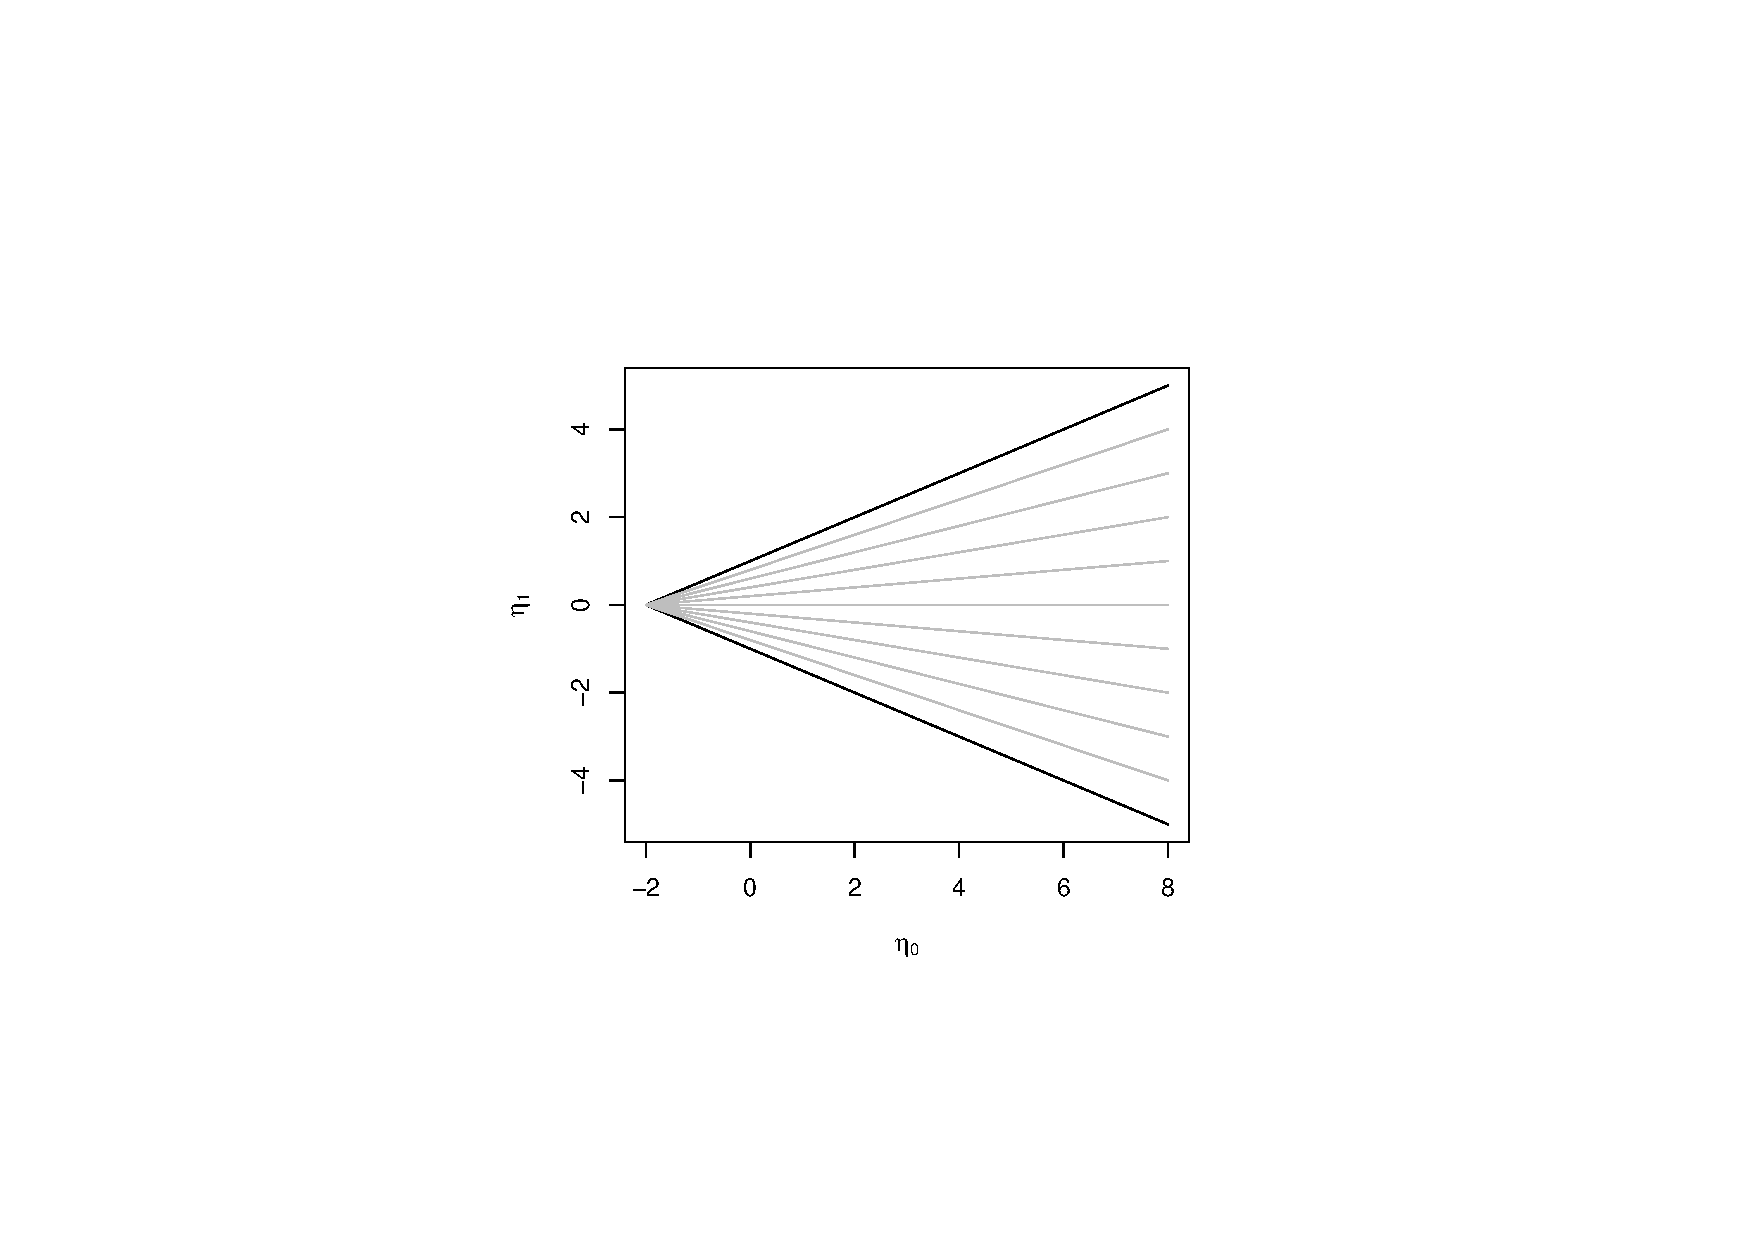
\includegraphics[trim = 80mm 45mm 80mm 60mm, clip, width=0.7\textwidth]{R/boatshape-domain}%
%}
\caption[Bounds for the domain of $\eta_0$ and $\eta_1$ for the Beta-Binomial model,
with rays of constant expectation for $y_c = \{0.1,0.2,\ldots,0.9\}$.]%
{Bounds for the domain of $\eta_0$ and $\eta_1$ for the Beta-Binomial model (black),
with rays of constant expectation for $y_c = \{0.1,0.2,\ldots,0.9\}$ (grey).}
\label{fig:boatshape-domain}
\end{figure}

While $\yz$ had the convenient property of being equal to
the prior expectation of the mean sample statistic $\ttau(x)$ (here, $\ttau(x) = s/n$),
%$\E\big[\E[\ttau(x) \mid \psi] \mid \nz, \yz\big]$,
$\eta_1$ is only slightly more difficult to interpret.
From \eqref{eq:trafotony} we can derive that points $(\eta_0,\eta_1) \in \Eta$
on rays emanating from the coordinate $(-2,0)$,
i.e., coordinates satifying
\begin{align}
\label{eq:raysofconstantexpectation}
\eta_1 = f(\eta_0) &= (\eta_0 + 2)(y_c - \frac{1}{2}) 
\end{align}
will have a constant expectation of $y_c$.
The domain $\Eta$, and these \emph{rays of constant expectation} emanating from the coordinate $(-2,0)$,
are depicted in Figure~\ref{fig:boatshape-domain}.


%\section{A Parameter Set Shape for Strong Prior-Data Agreement Modelling}

%\subsection{Informal Rationale for Boat-Shaped Parameter Sets}
\section{Parameter Sets and Imprecision in the Novel Parametrisation}
\label{boatshape-rationale}

In the parametrisation in terms of $(\nz,\yz)$ and $(\nn, \yn)$,
posterior inferences become more precise,
because the stretch in the main parameter dimension $y$, denoted by $\Delta_y(\PN)$,
tends to $0$ for $n \to \infty$ (see the discussion in Section~\ref{sec:ip-conjugateframework}).
In the domain $\Eta$ as depicted in Figure~\ref{fig:boatshape-domain},
instead the rays of constant expectation fan out for growing $n$, %**move outwards to the right,
while a parameter set will retain its size in updating.
Increased precision in a posterior parameter set $\EN$, which is just
its prior counterpart $\EZ$ shifted to the right,
is given by the fact the more $\EN$ is located to the right,
the fewer rays of constant expectation $\EN$ will intercept.
Imprecision in terms of $\E\big[\E[\ttau(x) \mid \psi] \mid \nn, \yn\big] = \yn$
can thus be imagined as the size of the `shadow' that a set $\EN$ casts
when considering a light source in $(-2,0)$ (the point from which the rays of constant expectation emanate).
In short, the smaller this shadow, the more precise the inferences.

In the context of the model from Section~\ref{sec:miksworld},
we will denote by $\ynl$ and $\ynu$ the bounds of this shadow,
i.e.,
\begin{align*}
\ynl &:= \min_{(\ezn,\eon) \in \EN} \yn = \min_{(\ezn,\eon) \in \EN} \frac{\eon}{\ezn+2} + \frac{1}{2}\,, \\
\ynu &:= \max_{(\ezn,\eon) \in \EN} \yn = \max_{(\ezn,\eon) \in \EN} \frac{\eon}{\ezn+2} + \frac{1}{2}\,,
\end{align*}
and we call the coordinates $\arg\min_{(\eta_0,\eta_1) \in \EN} \yn$ and $\arg\max_{(\eta_0,\eta_1) \in \EN} \yn$
the \emph{lower} and \emph{upper touchpoints} of $\EN$ responsible for the shadow $[\ynl, \ynu]$.
Mutatis mutandis, the same definitions can be made for the prior set $\EZ$.

Due to the fanning out of rays, most shapes for $\EZ$ will lead to decreasing imprecision for increasing $n$.
Indeed, models of type~(\ref{enum:modeltypes-a}),
where $\PZ = \nz \times [\yzl, \yzu]$,
are represented here again by a line segment $\EZ = \ezz \times [\eozl,\eozu]$,
such that the posterior touchpoints are, for any $s$ and $n$, $(\ezn,\eonl)$ and $(\ezz,\eonu)$,
where $\eonl$ and $\eonu$ are the updated versions of $\eozl$ and $\eozu$, respectively.
Due to \eqref{eq:eta-update}, it holds that $\eonu-\eonl = \eozu-\eozl$;
therefore, imprecision decreases here because a line segment of fixed size
will cast a smaller shadow when further to the right,
as illustrated in Figure~\ref{fig:boatshape-vertical}.

\begin{figure}  %trim=l b r t
\centering
%\fbox{%
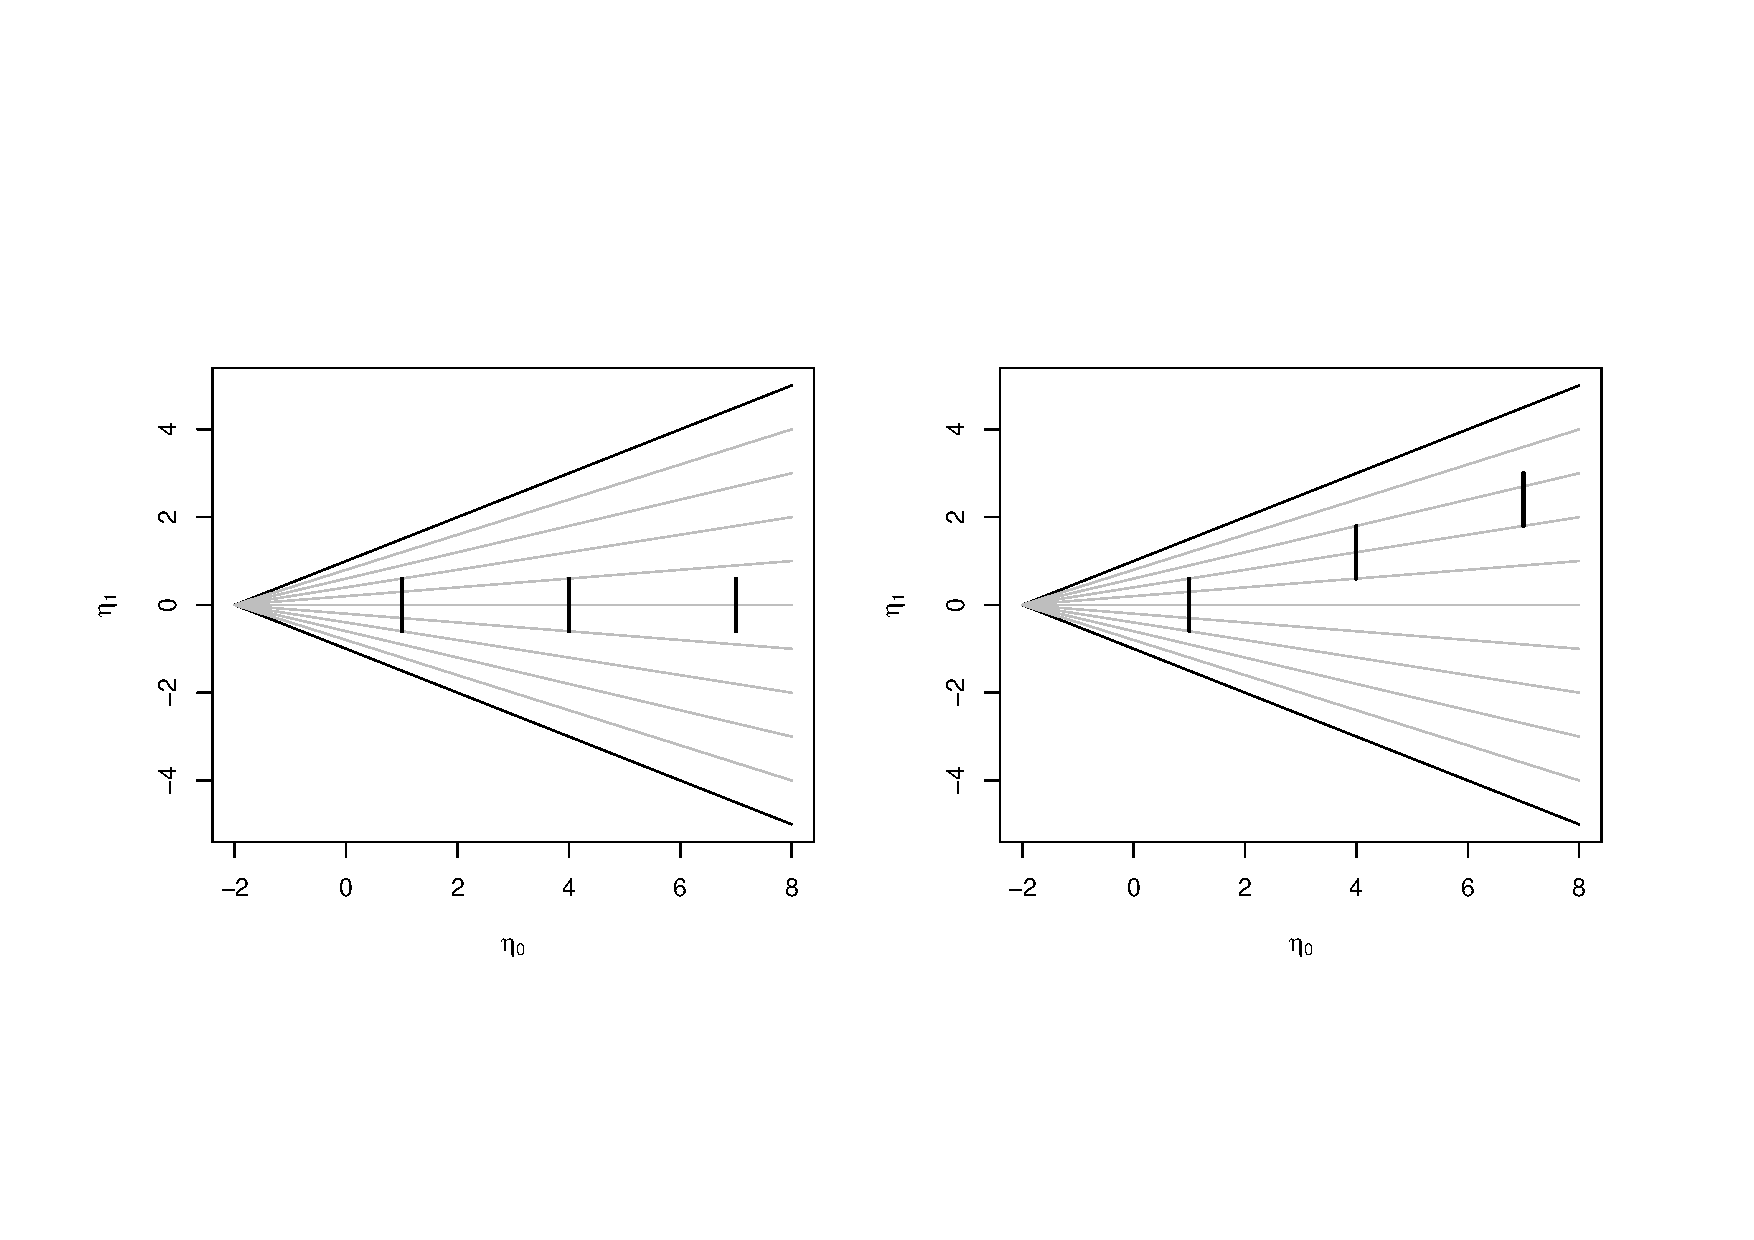
\includegraphics[trim = 15mm 45mm 25mm 60mm, clip, width=\textwidth]{R/boatshape-vertical}%
%}
\caption[Line segment parameter set $\EZ$ %
and respective posterior sets for $s/n=0.5$ and $s/n=0.9$.]%
{Prior parameter set $\EZ = \ezz \times [\text{\underline{$\eta$}${}_1\uz$},\eozu]$ and respective posterior sets $\EN$
for $s/n=0.5$ (left) and $s/n=0.9$ (right). Note that all sets have the same size,
imprecision decreasing only through their position on the $\eta_0$ axis.}
\label{fig:boatshape-vertical}
\end{figure}

For \pdc\ sensitivity, we need shapes that cover a range of $\eta_0$ values,
for the same reasons as in the framework of Section~\ref{sec:ip-conjugateframework},
where only sets with a range of $\nz$ values offered this property.
Sets that are elongated along the rays of constant expectation
will behave here similar to the rectangular shapes of Section~\ref{sec:ip-conjugateframework}.
When shifted along its respective ray of constant expectation,
imprecision will be reduced as the shadow of the set will become smaller just as described above for line segments.
When such a shape is instead shifted away from its ray of constant expectation,
imprecision will be increased, as a prolonged shape that is now turned away from its ray 
will cast a larger shadow.%
\footnote{This will become clear from the depiction of boatshape sets in Figure~\ref{fig:boatshape-posterior-mik}.} 

A set $\EZ$ allowing for less imprecison in case of strong prior-data agreement
must also be able to cast a smaller shadow if the update shift goes into the direction of its ray,
%of $s/n$ according the information,
but we will enhance this effect by considering now also the properties
of the canonical posteriors the coordinates of $\EN$ represent.

We have seen that for the conjugate distributions themselves,
$\nz$ is generally a parameter determining the spread of the distribution
(e.g., in the Normal-Normal model (see Section~\ref{sec:norm-norm}), $\nz$ was the inverse variance),
such that we will have more precise inferences if the shadow bounds $\ynl$ and $\ynu$
are attained at higher values of $\eta_0$, leading to lower variances in the
`critical' distributions at the boundary of the posterior expectation interval $[\ynl,\ynu]$.
For this to happen, we need a shape for which the touchpoints responsible for $\ynl$ and $\ynu$
are attained at higher values of $\eta_0$ in case of strong prior-data agreement.
Shapes that accomplish this must have a curvature along their length in the direction
of the constant rays of expectation.
The shape we suggest thus looks like a bullett, or like a boat with a transom stern
(see, e.g., Figure~\ref{fig:boatshape-prior}).

\section{The Boatshape}
\label{sec:boatshape-2}

In this section, %~\ref{sec:boatshape-2} below,
%Now,
we will suggest a parametrisation for such a shape.
The definition, along with some first graphical examples, is given in Section~\ref{sec:basicdefboat},
and we discuss some first technical results for this shape in Sections~\ref{sec:touchpoints} -- \ref{sec:generalupdate}.


\subsection{Basic Definition}
\label{sec:basicdefboat}

We will now present a parametrisation for such a boat-shaped parameter set $\EZ$.
To keep things simple, we will consider here and in the follwing only prior sets
that are symmetric around the $\eta_0$ axis, i.e., centered around $y_c = 0.5$,
expressing the prior information that we deem a fraction of successes of $\frac{s}{n} = \frac{1}{2}$
as the most probable.%
\footnote{The general case of sets $\EZ$ with central ray $y_c \neq 0.5$
is discussed informally in Section~\ref{sec:boatshape-outlook}.}

For the contours of $\EZ$, we suggest an exponential function as the functional form,
where the `prow' of the set is located at $(\ezl, 0)$.
The lower and the upper contour $\czl(\eta_0)$ and $\czu(\eta_0)$ are defined as
\begin{align*}
\czl(\eta_0) &= -a \left( 1 - e^{-b(\eta_0 - \ezl)} \right)\,, \\
\czu(\eta_0) &= \phantom{-}%
                 a \left( 1 - e^{-b(\eta_0 - \ezl)} \right)\,, 
\end{align*}
where $a$ and $b$ are parameters controlling the shape.
We will also need the respective derivations with respect to $\eta_0$, given by
\begin{align*}
\frac{d}{d\eta_0} \czl(\eta_0) &= -ab e^{-b(\eta_0 - \ezl)}\,, \\
\frac{d}{d\eta_0} \czu(\eta_0) &= \phantom{-}%
                                   ab e^{-b(\eta_0 - \ezl)}\,.
\end{align*}
For this basic situation, given the parameters $\ezl$, $\ezu$, $a$, and $b$,
$\EZ$ is thus defined as
\begin{align}
\label{eq:basicset}
\EZ =
\{(\eta_0,\eta_1) \colon \ezl \le \eta_0 \le \ezu, \czl(\eta_0) \le  \eta_1 \le \czu(\eta_0) \}\,.
\end{align}
A prior boatshape set with $\ezl=1$, $\ezu=6$, $a=2$, and $b=0.8$ is depicted in Figure~\ref{fig:boatshape-prior},
where the left graph shows this set as defined in terms of $(\eta_0,\eta_1)$,
and the right graph shows the set from the left transformed into the space $\N \times \Y$.

\begin{figure}  %trim=l b r t
\centering
%\fbox{%
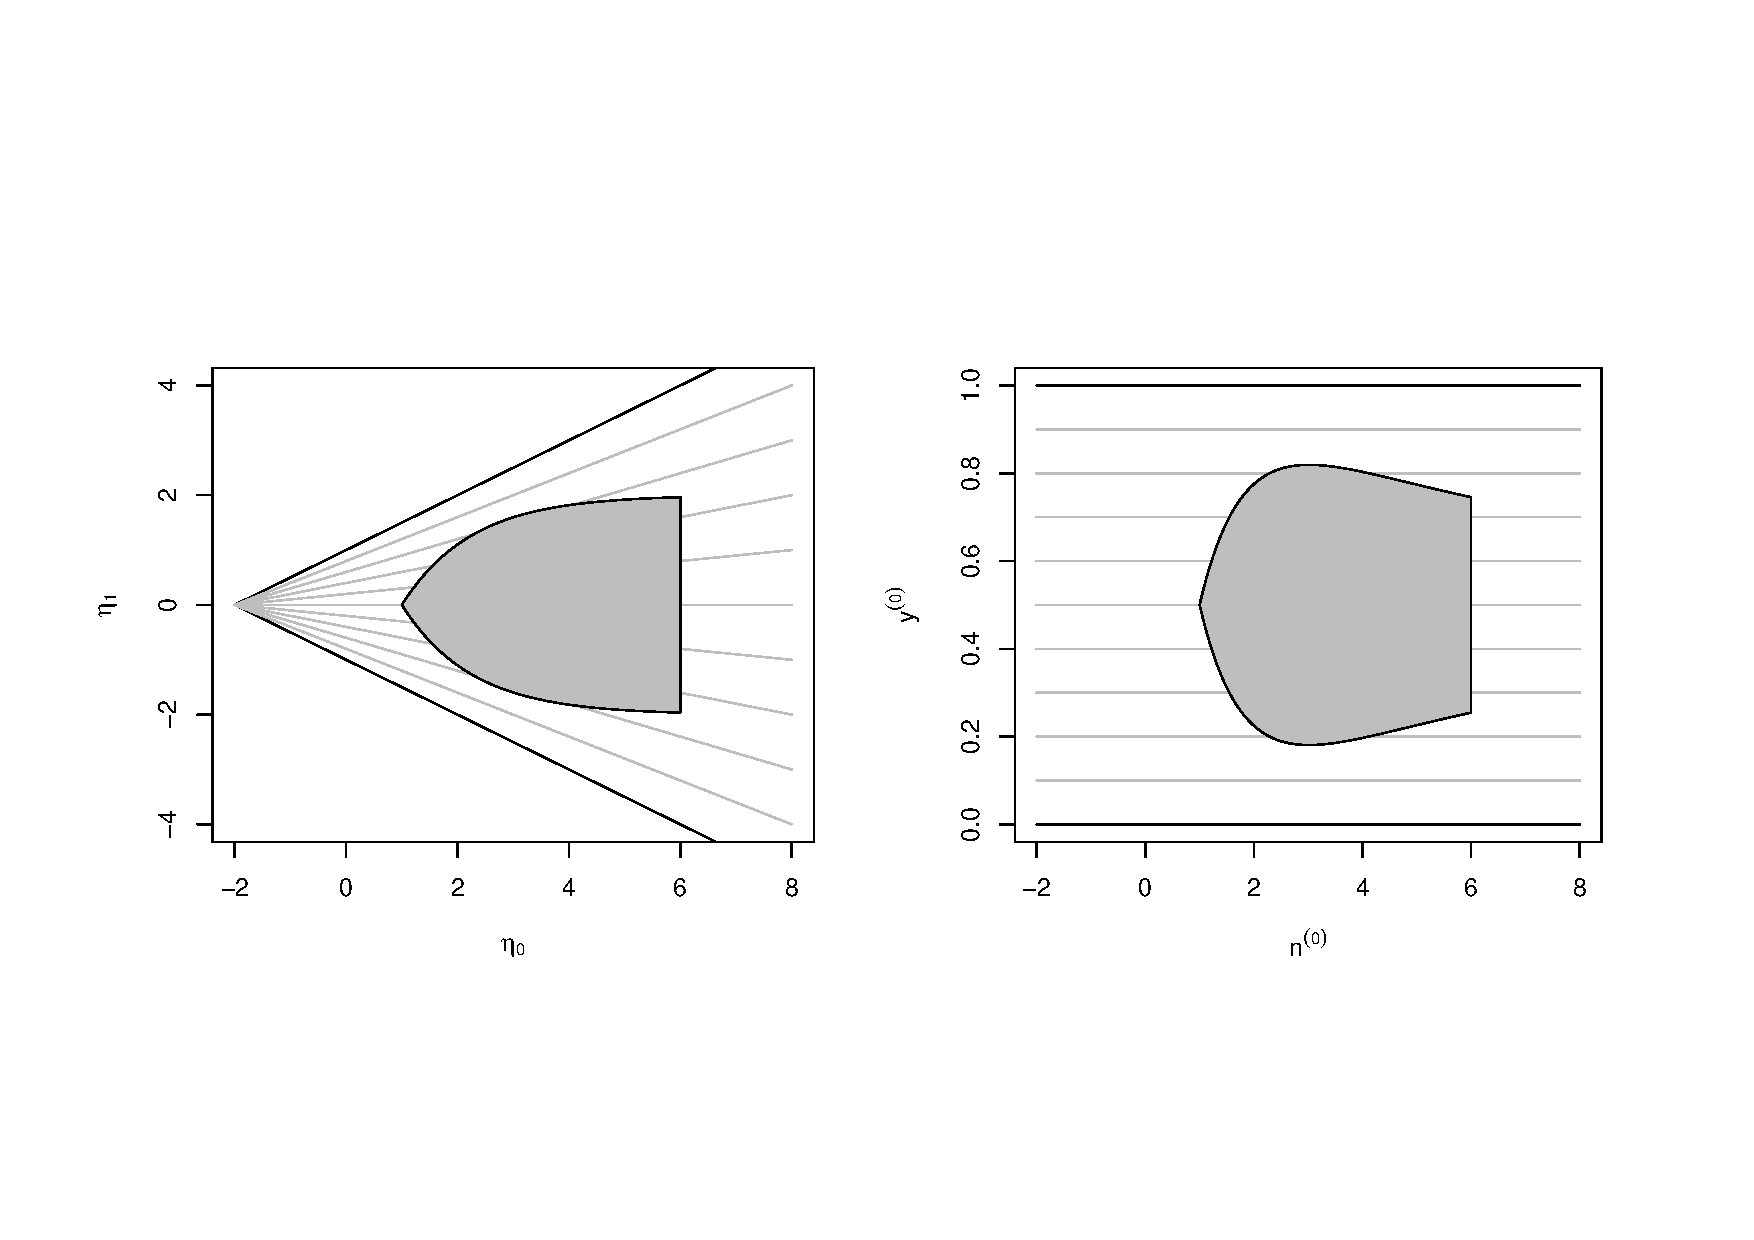
\includegraphics[trim = 15mm 45mm 25mm 60mm, clip, width=\textwidth]{R/boatshape-prior}%
%}
\caption[Boatshape prior set in the parametrisation via $(\eta_0,\eta_1)$ and via $(\nz,\yz)$.]%
{Boatshape prior set in the parametrisation via $(\eta_0,\eta_1)$ (left) and via $(\nz,\yz)$ (right),
with parameters $\ezl=1$, $\ezu=6$, $a=2$, and $b=0.8$.}
\label{fig:boatshape-prior}
\end{figure}


We have as yet no appealing formal description for the role of the parameters $a$ and $b$. %that,
%togeher with $\ezl$ and $\ezu$, define the boat-set (see Section~\ref{sec:basicdefboat} below).
Informally, $a$ determines the half-width of the set;
the width, i.e., the size in the $\eta_1$ dimension, would be $a$ if $\ezu \to \infty$.
$b$ instead determines the `bulkyness' of the shape.
Together with $\ezl$, $a$ and $b$ determine the prior interval for the expected success probability $[\yzl, \yzu]$.
For fixed $\ezl$ and $a$, increasing $b$ leads to a wider prior expectation interval.
For $[\yzl, \yzu]$, the choice of $\ezu$ is irrelevant.%
\footnote{$\ezu$ plays only a role in determining when the `unhappy learning' phase starts
(see end of Section~\ref{sec:generalupdate}).}


\begin{figure}  %trim=l b r t
\centering
%\fbox{%
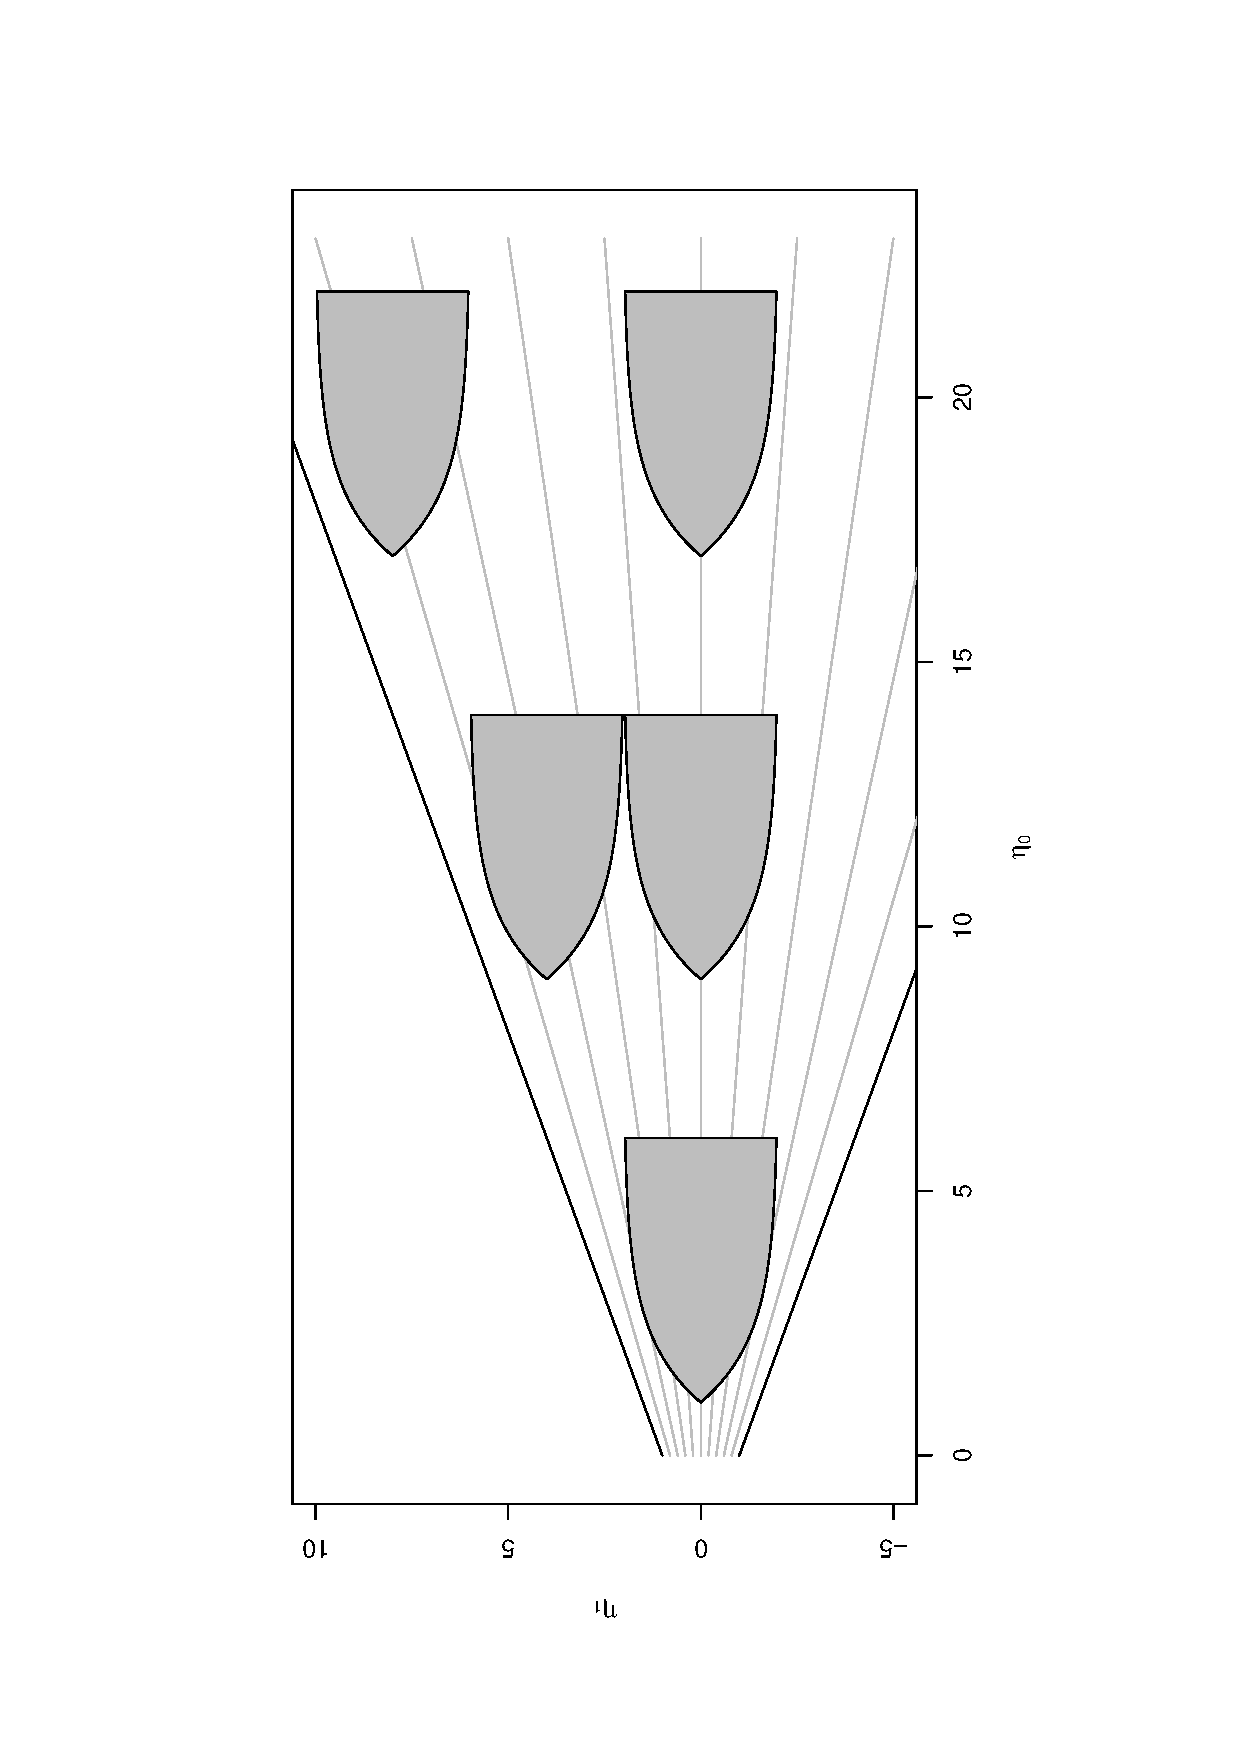
\includegraphics[trim = 20mm 35mm 30mm 45mm, clip, width=\textwidth]{R/boatshape-posterior-mik}%
%}
\caption[Boatshape prior and posterior sets for data in accordance and in conflict with the prior.]%
{Boatshape prior and posterior sets for data in accordance and in conflict with the prior.
The prior set is the same as in Figure~\ref{fig:boatshape-prior}.
While the posterior sets for $\frac{s}{n}=0.5$ move along the ray for $y_c=0.5$,
the posterior sets for $\frac{s}{n}=1$ are shifted away from the ray for $y_c=0.5$,
resulting in increased posterior imprecision.
Note that lower and upper touchpoints are in the middle of the contour
for the prior and the posterior resulting for data $\frac{s}{n}=\frac{4}{8}$,
while at least one touchpoint is at the end for all other sets.
(see also Figure~\ref{fig:boatshape-posterior-normal}).}
\label{fig:boatshape-posterior-mik}
\end{figure}


\begin{figure}  %trim=l b r t
\centering
%\fbox{%
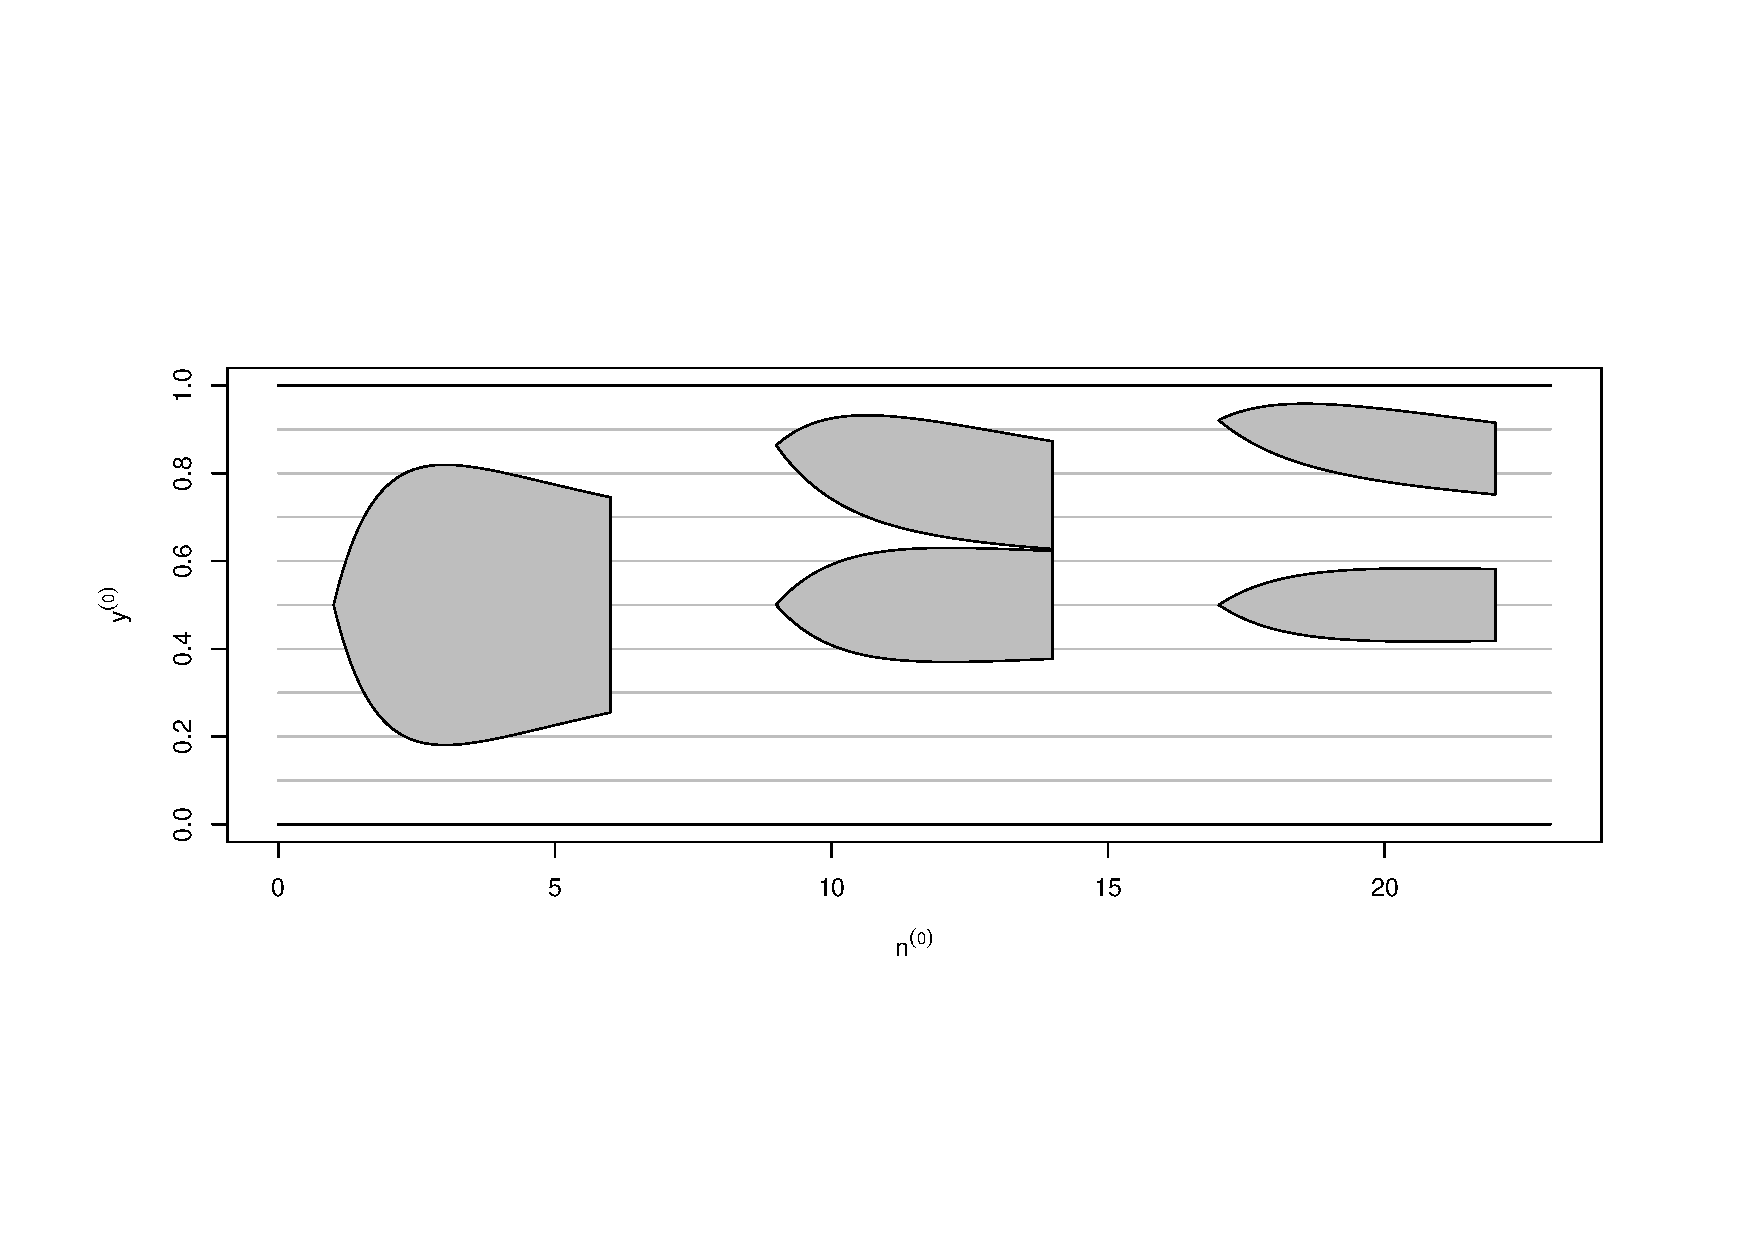
\includegraphics[trim = 15mm 45mm 25mm 60mm, clip, width=\textwidth]{R/boatshape-posterior-normal}%
%}
\caption[Boatshape prior and posterior sets from Figure~\ref{fig:boatshape-posterior-mik} in the parametrisation via $(\nz,\yz)$.]%
{Boatshape prior and posterior sets from Figure~\ref{fig:boatshape-posterior-mik} in the parametrisation via $(\nz,\yz)$.
Note that in the strong prior-data agreement case,
posterior sets based on a rectangular prior set with the same prior main parameter imprecision
would be larger than the ones depicted here, illustrating the extra gain in precision.}
\label{fig:boatshape-posterior-normal}
\end{figure}


\subsection{Finding the Touchpoints for the Basic Set}
\label{sec:touchpoints}

In contrast to models in the parametrization discussed in Section~\ref{sec:ip-conjugateframework},
where $\yzl$ and $\yzu$ were at either ends of a set $\PZ$,
here, for a set \eqref{eq:basicset}, the touchpoints $\yzl$ and $\yzu$ 
are not necessarily at $\ezzl$ or $\ezzu$.%
\footnote{See, e.g., the prior in Figure~\ref{fig:boatshape-prior}.}
Instead, the rays of constant expectation \eqref{eq:raysofconstantexpectation}
touching the parameter set must be determined to find $\yzl$ and $\yzu$.
To do this, the tangent equations for the lower and the upper contour function
depending on $\eta_0$ are determined.
As all rays of constant expectation pass through the point $(-2,0)$,
the tangent that passes through this point is determined by inserting this point
into the tangent equation, and the resulting equation is solved for $\eta_0$.
The resulting points $(\eta_0^l,\czl(\eta_0^l))$ and $(\eta_0^u,\czu(\eta_0^u))$
then give the lower and upper touchpoints of the parameter set, respectively,
and can be transformed to $\yzl$ and $\yzu$ by using \eqref{eq:trafotony}.

As the basic set is symmetrical to the $\eta_0$ axis, we have $\eta_0^u = \eta_0^l$,
and it suffices to find, e.g., $\eta_0^u$, by considering the upper contour tangent.

We denote the tangent in contour point $(\eta_0,\czu(\eta_0))$ by
\begin{align*}
\ol{t}_{\eta_0}(x) &= dx + i\,,
\end{align*}
where $d = \frac{d}{d\eta_0} \czu(\eta_0)$ and
$i$ such that $\ol{t}_{\eta_0}(x)$ goes through the point $(\eta_0,\czu(\eta_0))$:
\begin{align*}
\ol{t}_{\eta_0}(x) &= dx + i \quad \Longleftrightarrow\\
\czu(\eta_0) &= \frac{d}{d\eta_0} \czu(\eta_0) \eta_0 + i \\
i &= \czu(\eta_0) -\frac{d}{d\eta_0} \czu(\eta_0) \eta_0 \\
  &= a - a e^{-b(\eta_0 - \ezl)} - \eta_0 ab e^{-b(\eta_0 - \ezl)} \\
  &= a - a (1 + b \eta_0) e^{-b(\eta_0 - \ezl)} \\
\Longrightarrow\quad
\ol{t}_{\eta_0}(x) &= ab e^{-b(\eta_0 - \ezl)} x + a - a (1 + b \eta_0) e^{-b(\eta_0 - \ezl)} \\
                   &= a - a \big(1 + b(\eta_0-x)\big) e^{-b(\eta_0 - \ezl)}
\end{align*}
Now, let us find the touchpoint $(\eta_0^u, \czu(\eta_0^u))$ whose tangent goes through $(-2,0)$, as this gives us $\yzu$.
We insert $(-2,0)$ into the tangent equation and solve for $\eta_0$.
\begin{align}
a - a \big(1 + b(\eta_0^u + 2)\big) e^{-b(\eta_0^u - \ezl)} &\stackrel{!}{=} 0 \nonumber\\
1 + b(\eta_0^u + 2) &\stackrel{!}{=} e^{b(\eta_0^u - \ezl)} \label{eq:eta0u}
\end{align}
This equation has only one solution for $\eta_0^u > \ezl$, that is,
however, not available in closed form.

As a general rule, the nearer $\eta_0^u$ is to $\ezl$, the larger $\frac{d}{d\eta_0} \czu(\eta_0^u)$,
that is, $\yzu$ %the upper expected value for the prior set
is more away from $\frac{1}{2}$.
Here, this means that the larger $\eta_0^u$, the more imprecise is the prior parameter set.


\subsection{Strong Prior-Data Agreement Property}
\label{sec:spda-property}

We will now prove the essential property that sets \eqref{eq:basicset}
will lead to especially precise inferences when data are strongly suporting prior information.

For a prior parameter set $\EZ = \ezz \times [\eozl,\eozu]$
%, with $\eta_0 = \ezz$ fixed and $\eta_1$ varying in an interval $[\eol, \eou]$
symmetric around $0$,
the prior upper expected value $\yzu$
results from the transformation \eqref{eq:trafotony} of the point $(\ezz,\eozu)$.
The posterior upper expected value $\ynu$,
given data that coincide especially well with the prior,
i.e., data with $s = \frac{n}{2}$, will then be found at the point $(\ezz+n,\eozu)$,
because in this case, the set does not move in the vertical ($\eta_1$) direction.
As $\yz$ is decreasing in $\eta_0$ and $\eta_1$ is constant, $\ynu$ %the posterior upper expected value
will be lower than $\yzu$, i.e., imprecision is reduced.

Imprecision is, however, even more strongly reduced for the boatshape parameter set \eqref{eq:basicset}.
Say, we define the prior parameter set such that the prior upper touchpoint
is at the $\eta_0$ coordinate $\eta_0^u = \ezz$.
For this shape, the $\eta_0$ coordinate for the posterior upper touchpoint ${\eta_0^u}\un$
will be  larger than the updated $\ezz$, i.e., ${\eta_0^u}\un > \ezz + n$ (as will be shown below), and thus $\ynu$ is lower.
Although the $\eta_1$ coordinate will be slightly larger at the point $({\eta_0^u}\un, \ol{c}({\eta_0^u}\un))$
as compared to the point $(\ezz+n,\eozu)$, the corresponding $\ynu$ is still lower,
as it holds that
\begin{align*}
\frac{d}{d\eta_0} \ol{c}({\eta_0^u}\un) < \frac{d}{d\eta_0} \ol{c}(\ezz + n)
\end{align*}
because $\frac{d}{d\eta_0} \ol{c}(\eta_0)$ is decreasing in $\eta_0$,
and a smaller slope for the tangent through $(-2,0)$ is equivalent to a lower $\ynu$.
This is the desired reduction in imprecision for the case of strong prior-data agreement,
also depicted exemplarily in Figures~\ref{fig:boatshape-posterior-mik} and \ref{fig:boatshape-posterior-normal}.

The property ${\eta_0^u}\un > \ezz + n$ of the boatshape set will be shown below.
Due to symmetry of prior and posterior parameter shape around the $\eta_0$ axis,
${\eta_0^u}\un = {\eta_0^l}\un$, i.e.,
the touchpoint at the upper contour (giving $\ynu$) is equal to
the touchpoint at the lower contour (giving $\ynl$),
and thus, the argument formulated in terms of ${\eta_0^u}\un$ holds also for ${\eta_0^l}\un$.

The upper exponential contour for the posterior boatshape,
updated with $s = \frac{n}{2}$, has its `prow' now at $(\ezl + n, 0)$,
and is defined by the function
\begin{align*}
\ol{c}(\eta_0) &= a \left( 1 - e^{-b(\eta_0 - n -\ezl)} \right) \\
\frac{d}{d\eta_0} \ol{c}(\eta_0) &= ab e^{-b(\eta_0 - n - \ezl)} \,.
\end{align*}
The tangent in contour point $(\eta_0,\ol{c}(\eta_0))$ is
\begin{align*}
\ol{t}_{\eta_0}(x) &= a - a \big(1 + b(\eta_0-x)\big) e^{-b(\eta_0 - n - \ezl)} \,.
\end{align*}
Again, we insert $(-2,0)$ into this tangent equation and solve for $\eta_0$.
\begin{align}
a - a \big(1 + b({\eta_0^u}\un + 2)\big) e^{-b({\eta_0^u}\un - n - \ezl)} &\stackrel{!}{=} 0 \nonumber\\
1 + b({\eta_0^u}\un + 2) &\stackrel{!}{=} e^{b({\eta_0^u}\un - n - \ezl)} \,.\label{eq:eta0uposterior}
\end{align}
We compare now \eqref{eq:eta0uposterior} to \eqref{eq:eta0u} and conclude
that indeed ${\eta_0^u}\un > \ezz + n$:
\begin{figure}
\centering
%\fbox{
%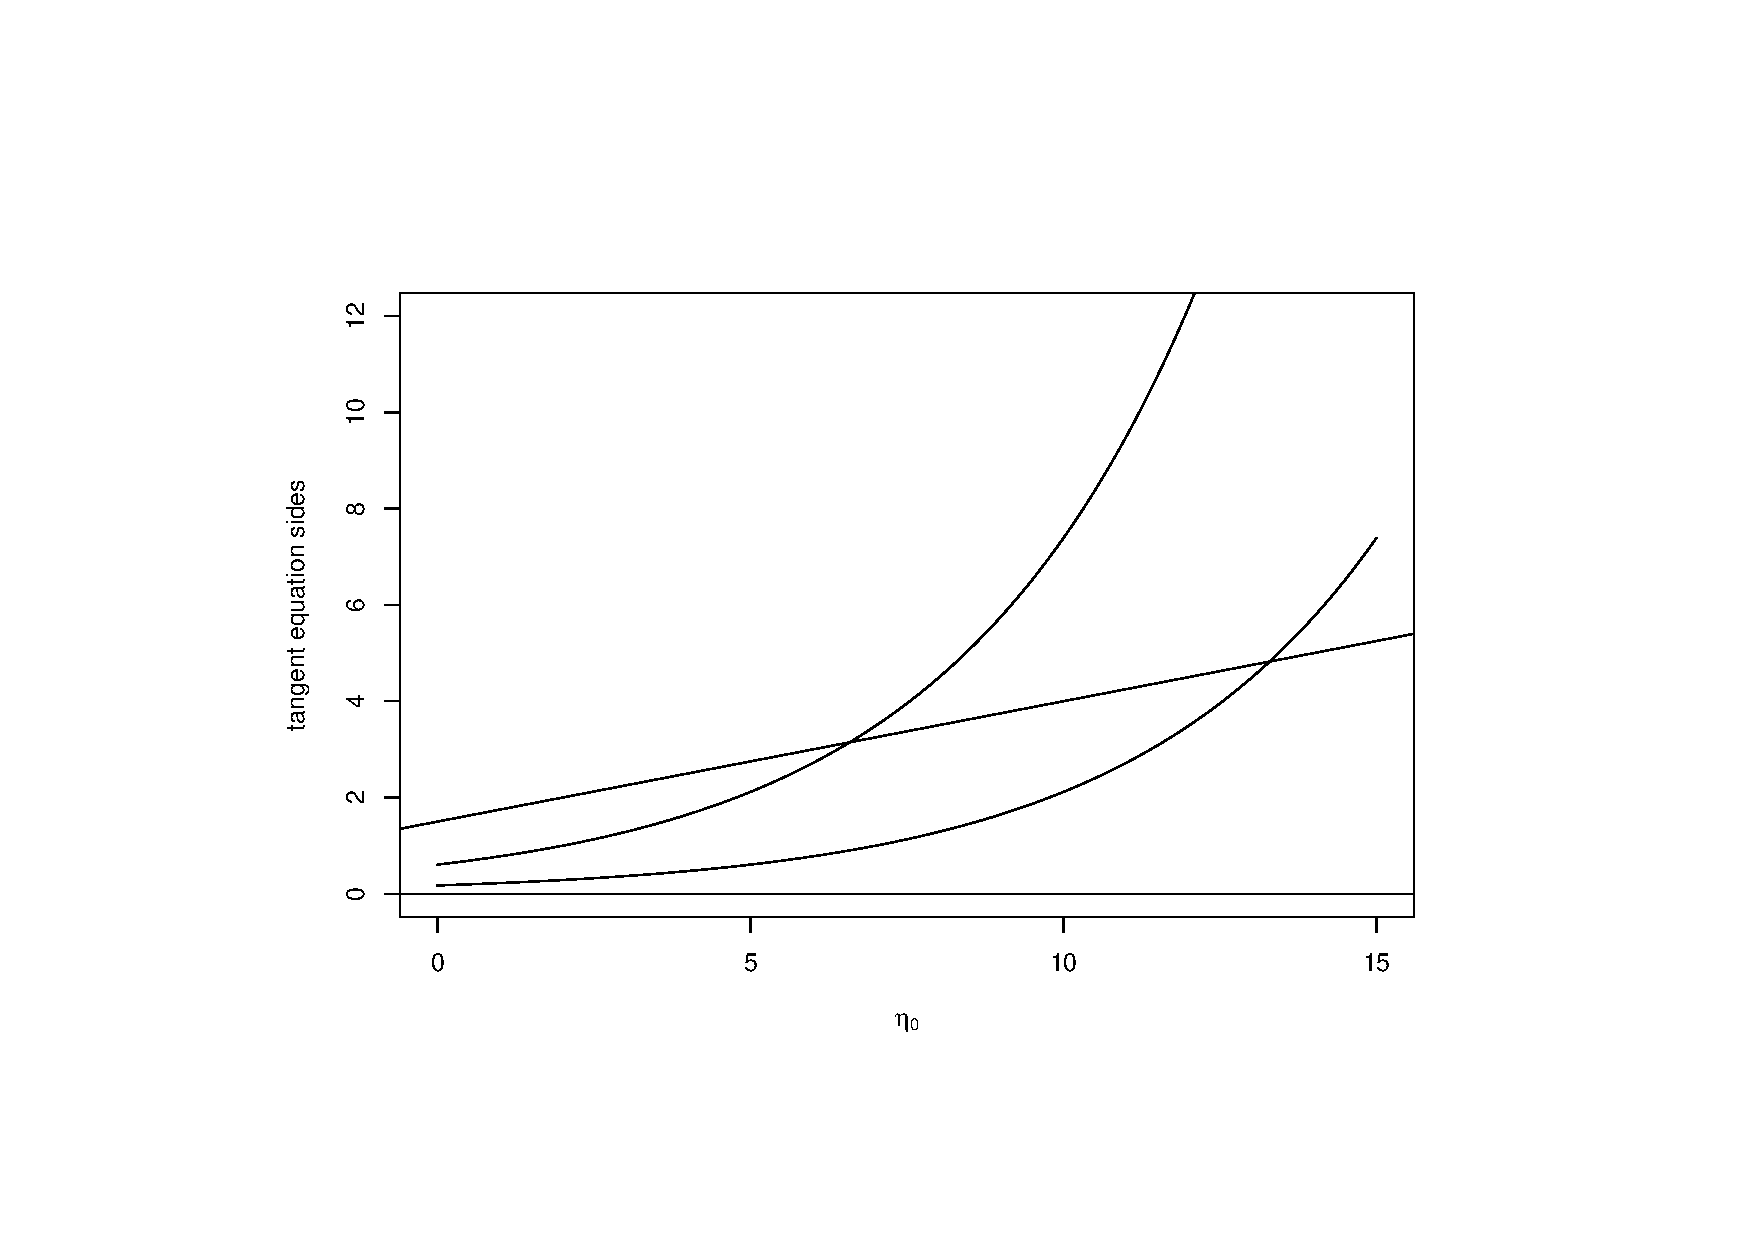
\includegraphics[trim = 45mm 35mm 45mm 45mm, clip, width=\textwidth]{R/prior-vs-posterior-eta0u}%
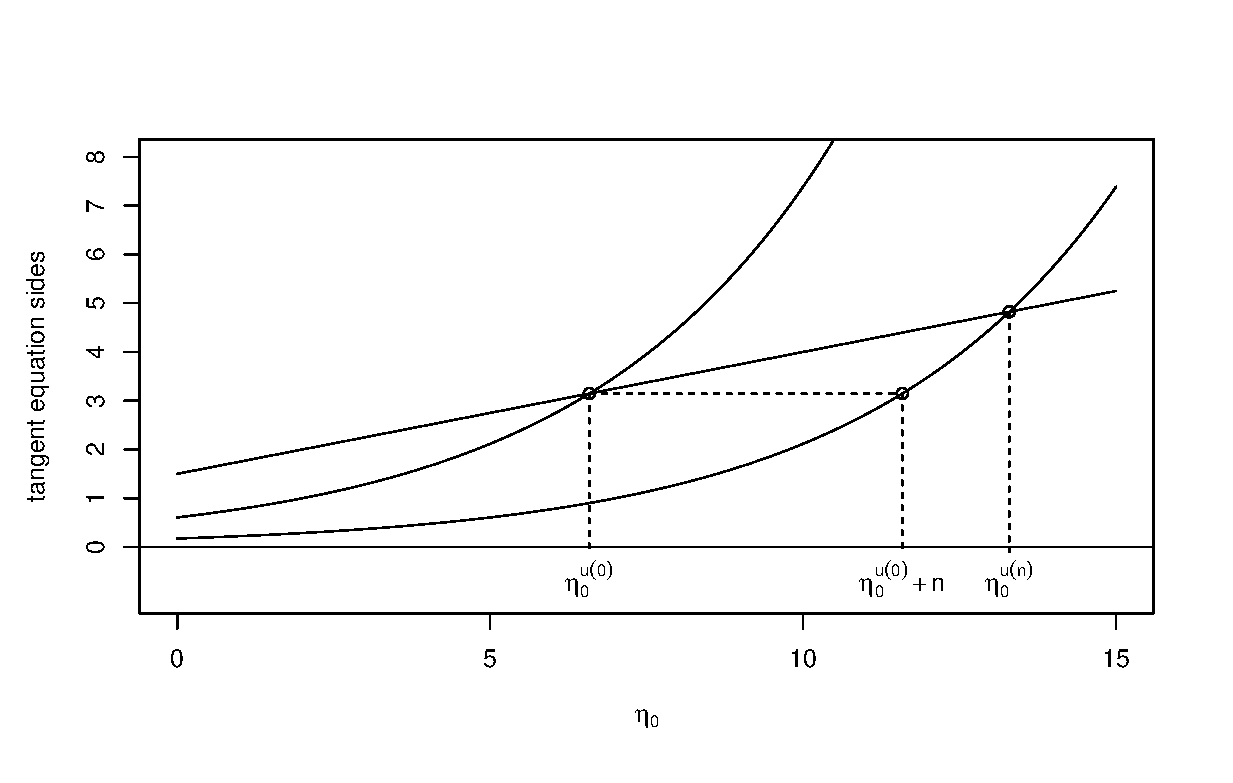
\includegraphics[width=\textwidth]{R/prior-vs-posterior-eta0u.eps}
%}
\caption{Illustration for the argument that ${\eta_0^u}\un > {\eta_0^u}\uz + n$.}
\label{fig:spda1}
\end{figure}
In Figure~\ref{fig:spda1}, the two exponential graphs 
represent the right hand side of equations \eqref{eq:eta0u} and \eqref{eq:eta0uposterior}.
Both have the same curvature; the right one is the same as the left, only being shifted to the right by $n$.
The left hand side of \eqref{eq:eta0u} and \eqref{eq:eta0uposterior} coincides and is the linear function.
$\ezz$ and $\ezn$ are determined by the intersection of the linear with the exponential graphs.
$\ezz + n$ is thus on the right exponential curve, being $\ezz$ shifted to the right by $n$.
Because ${\eta_0^u}\un$ results from the intersection of the right exponential curve and the linear function,
it is necessarily larger than ${\eta_0^u}\uz + n$, as the linear function is increasing.

***also: the larger the bulkyness parameter $b$, the steeper the linear function
and thus the larger the distance of ${\eta_0^u}\un$ to ${\eta_0^u}\uz + n$,
that is, the stronger the prior-data agreement effect of the shape.
Can see this also from normalworld***: a bulkyer the shape has more ueberhang
which gets reduced by updating as it is located towards the left side of the set***

\subsection{General Update with \texorpdfstring{$s > \frac{n}{2}$}{s > n/2}}
\label{sec:generalupdate}

Let us now consider the update of the basic boatshape \eqref{eq:basicset} %symmetric around the $\eta_0$ axis,
in the general case $s \neq \frac{n}{2}$.
Due to symmetry of the prior set, we can, without loss of generality,
consider again only the case $s > \frac{n}{2}$.

For the prior set, being symmetric around the $\eta_0$ axis,
both touchpoints are located at the same $\eta_0$ coordinate,
the resulting $\yzl$ and $\yzu$ having the same distance to $0.5$.
Regarding the posterior set, according to \eqref{eq:eta-update},
$\eta_0$ coordinates are incremented by $n$, while
$\eta_1$ coordinates are incremented by $s+\frac{n}{2}$.
That is, if $s \neq \frac{n}{2}$, the updated set is no longer symmetric around the $\eta_0$ axis,
such that we must consider the lower and upper contours separately.

The upper and lower contours and their respective derivatives for the updated boatshape set are now
\begin{align*}
\ol{c}(\eta_0)                   &= s - \frac{n}{2} + a - a e^{-b(\eta_0 - n - \ezl)} \,,\\
\frac{d}{d\eta_0} \ol{c}(\eta_0) &=                      ab e^{-b(\eta_0 - n - \ezl)} \,,\\
\ul{c}(\eta_0)                   &= s - \frac{n}{2} - a + a e^{-b(\eta_0 - n - \ezl)} \,,\\
\frac{d}{d\eta_0} \ul{c}(\eta_0) &=                     -ab e^{-b(\eta_0 - n - \ezl)} \,.
\end{align*}
The upper and lower tangents in contour point $(\eta_0,c(\eta_0))$ are now given by
\begin{align*}
\ol{t}_{\eta_0}(x) &= s - \frac{n}{2} + a - a \big(1 + b(\eta_0-x)\big) e^{-b(\eta_0 - n - \ezl)} \,,\\
\ul{t}_{\eta_0}(x) &= s - \frac{n}{2} - a + a \big(1 + b(\eta_0-x)\big) e^{-b(\eta_0 - n - \ezl)} \,.
\end{align*}
Inserting again $(-2,0)$, we get the equations defining the $\eta_0$ coordinates
${\eta_0^u}\un$ and ${\eta_0^l}\un$
that give us $\ynu$ and $\ynl$, respectively:
\begin{align}
%s - \frac{n}{2} + a - a \big(1 + b(\eta_0^u + 2)\big) e^{-b(\eta_0^u - n - \ezl)} &\stackrel{!}{=} 0 \nonumber\\
\label{eq:eta0u-general}
\frac{a}{s - \frac{n}{2} + a} \big(1 + b(\eta_0^u + 2)\big) &\stackrel{!}{=} e^{b(\eta_0^u - n - \ezl)} \,,\\
\label{eq:eta0l-general}
\frac{a}{\frac{n}{2} -s  + a} \big(1 + b(\eta_0^u + 2)\big) &\stackrel{!}{=} e^{b(\eta_0^u - n - \ezl)} \,.
\end{align}

We see thus that the picture from Figure~\ref{fig:spda1} holds here as well,
except that the linear function (left hand side of equations
\eqref{eq:eta0u-general} and \eqref{eq:eta0l-general}) is changed in slope and intercept by a factor.
(Equivalently, we can consider it to be rotated around the root $-2-\frac{1}{b}$.)
For $s=\frac{n}{2}$, this factor is 1 for both the lower and the upper touchpoint,
resulting in the situation of strong prior-data agreement as considered in Section~\ref{sec:spda-property},
where ${\eta_0^u}\un = {\eta_0^l}\un$ moved to the right.

Due to symmetry, we will consider the case $s > \frac{n}{2}$ only 
to describe ${\eta_0^u}\un$ and ${\eta_0^l}\un$.

\paragraph{Description of ${\eta_0^u}\un$.}

The factor to the linear function $\frac{a}{s - \frac{n}{2} + a}$
in \eqref{eq:eta0u-general} is smaller than $1$ and decreasing in $s$.
Thus, the larger $s$, the smaller the factor, the most extreme case being $s=n$,
where the factor is $\frac{a}{\frac{n}{2} + a}$.
As the linear function's slope will be less steep (the intercept is lowered as well),
%\footnote{The common root of the linear functions for any $s$ is at $\eta_0 = -2 -\frac{1}{b}$.}
the intersection with the exponential function moves to the left,
i.e.\ $\eta_0^u(s) < \eta_0^u(\frac{n}{2})$ for $\frac{n}{2} < s \le n$.
This means that $\ynu(s) > \ynu(\frac{n}{2})$ in general.
However, decrease of $\eta_0^u(s)$ is limited by $\ezl+n$.
When the intersection point reaches the left end of the shape at $\ezl+n$,
the gradual increase of $\ynu$ through the changing tangent slope 
for $\ezl+n \le \eta_0^u(s) \le \eta_0^u(\frac{n}{2})$ is replaced
by a different change mechanism,
where increase of $\ynu$ is solely due to increase in the $\eta_1$ direction.
Due to \eqref{eq:trafotony}, $\ynu$ is then linear in $s$.

\paragraph{Description of ${\eta_0^l}\un$.}

In \eqref{eq:eta0l-general}, the factor to the linear function is $\frac{a}{\frac{n}{2} - s + a}$.
Here, we have to distinguish the two cases $\frac{n}{2} \le s < \frac{n}{2} + a$
and $s \ge \frac{n}{2} + a$.
In the first case, the factor is larger than $1$ and increasing in $s$.
Therefore, the intersection of the linear function with the exponential function
will move towards the right, i.e., we will have a larger ${\eta_0^l}\un$, and $\ynl$ increases.
In the second case, the factor is undefined (for $s = \frac{n}{2} + a$)
or negative (for $s > = \frac{n}{2} + a$).
Either way, there will be no intersection of the linear function with the exponential function
for any $\eta_0 > \ezl + n$ (For $s \to \frac{n}{2} + a$, the slope $\to \infty$).
In fact, for $s \ge \frac{n}{2} + a$, the whole shape is above the $\eta_0$ axis,
and the touchpoint must be thus at $\ezu + n $.
Actually, $\ezu + n$ will be the touchpoint already at some $\frac{n}{2} \le s < \frac{n}{2} + a$,
when the intersection point arrives at $\ezu + n$.
At this point, gradual increase of $\ynl$ resulting from the movement of ${\eta_0^l}\un$ along the set
towards the right is replaced by a linear increase in $s$.
Again, this linear increase is due to the $\eta_1$ coordinate being incremented
according to \eqref{eq:eta-update},
and from \eqref{eq:trafotony} we see that $\ynl$ is linear in $\eta_1$.

%Contrary to the former consideration, the posterior boatshape set updated with $s > \frac{n}{2}$
%is not symmetric around the $\eta_0$ axis.
%To compare the posterior imprecision for $s=\frac{n}{2}$ with $s > \frac{n}{2}$,
%we have to consider also $\ynl$ for both cases.

%$\ynl(\frac{n}{2})$, i.e.\ the posterior lower expectation for $s=\frac{n}{2}$,
%can be found, due to symmetry around the $\eta_0$ axis, at ${\eta_0^l}\un = {\eta_0^u}\un$. 

\paragraph{Synthesis.}

For $s > \frac{n}{2}$, both $\ynu$ and $\ynl$ will at first increase gradually with $s$,
as ${\eta_0^u}\un$ moves to the left, and ${\eta_0^l}\un$ moves to the right.
We will call such updating of the prior parameter set,
where neither posterior touchpoints are at the left or the right end of the set, as `happy learning'.

At some $s^u$, ${\eta_0^u}\un$ will arrive at $\ezl + n$,
and at some $s^l$, ${\eta_0^l}\un$ will arrive at $\ezu + n$.
Whether $s^l < s^u$ or the other way round depends on
the choice of parameters $\ezl, \ezu, a$ and $b$.
Either way, once $s$ is larger than either of $s^l$ or $s^u$,
we switch to ``unhappy learning'',
where data $s$ is very much out of line with our prior expectations as expressed
by the prior parameter set $\EZ$.
Ultimately, when $s > s^u$ and $s > s^l$,
both $\ynu$ and $\ynl$ will increase linearly in $s$, but with different slopes.
$\ynu$ will increase with slope $\frac{1}{\ezl + n + 2}$,
whereas $\ynl$ will increase with a lower slope $\frac{1}{\ezu + n + 2}$.


\section{Example / Application?}
\label{sec:examples}

illustrate with simple inferences:\\
posterior mean $\E[\theta\mid\nn,\yn] = \yn$\\
posterior predictive $\p(s^*=1,n^*=1\mid \nn, \yn) = \yn$\\
$\modus(\theta\mid \nn, \yn) = \frac{\nn\yn -1}{\nn -2}$ (posterior mode)\\
$\p(s^*=2,n^*=2\mid \nn, \yn) = \yn \frac{\nn\yn + 1}{\nn + 1}$ (two successes in two future samples)\\
95\% credibility interval (symmetric or HPD? both must be derived numerically)

compare with Berger/Walley model with $s=1$, $s=2$, and rectangular set.

discuss briefly how to choose boatshape parameters.


\section{Conclusion and outlook}

***it's worth to study more shapes to cater for other objectives in inference behaviour

***more detailed study in elicitation of the boatshape set parameters necessary,
which should be done by pre-posterior analysis

***with the boatshape, we have a more flexible model for prior information
while remaining within the generalized Bayesian paradigm,
opening up a wide field for research

***aspects of design of experiments: Teddy paper (convincing another Bayesian)



%%%%%%%%%%%%%%%%%%%%%%%%%%%%%%%%%%%%%%%%%%%%%%%%%%%%%%%%%%%%%%%%%%%%%%%%%%%%%%%%
%% Bibliography and acknowledgements
%%%%%%%%%%%%%%%%%%%%%%%%%%%%%%%%%%%%%%%%%%%%%%%%%%%%%%%%%%%%%%%%%%%%%%%%%%%%%%%%

\bibliographystyle{ba}
\bibliography{boatpaper}


\begin{acknowledgement}
  The author(s) wish to thank....
\end{acknowledgement}

